%%%% Bachelorprojekt rapport %%%%
%%%% Elektronik Q3/Q4 2017 %%%%

% Kan anvendes til journaler eller afleveringer
\documentclass[11pt, a4paper, twoside, openany]{memoir}

\usepackage[utf8]{inputenc}		% Dansk input encoding (tegn)
\usepackage[english, danish]{babel}		% Danske formuleringer / orddeling
\usepackage[T1]{fontenc}		% Output-indkodning af tegnsaet (T1)


%%% Memoir indstillinger
%% Afstand mellem afsnit og videre
%% NIX PILLE - medmindre strengt nødvendigt
\setaftersubsubsecskip{6pt}	
\setbeforesubsubsecskip{6pt}
%\setaftersubsecskip{6pt}
%\setbeforesubsecskip{-\baselineskip}
%\setaftersecskip{6pt}
%\setbeforesecskip{-\baselineskip}
%\setaftersecskip{1ex}


\raggedbottom



\chapterstyle{section}

% ¤¤ Marginer ¤¤ %
\setlrmarginsandblock{3.5cm}{2.5cm}{*}		% \setlrmarginsandblock{Indbinding}{Kant}{Ratio}
\setulmarginsandblock{3.0cm}{2.5cm}{*}		% \setulmarginsandblock{Top}{Bund}{Ratio}
\checkandfixthelayout

%%% Font valg %%%
\usepackage{mathpazo}	%Palatinofont - matematikformler
\usepackage{eulervm}		%Palatinofont

%%% FIGURER OG TABELLER %%%
\usepackage{graphicx} 						% Haandtering af eksterne billeder (JPG, PNG, PDF)

\usepackage[export]{adjustbox}

\usepackage{subfig}

\usepackage{multirow}                		% Fletning af raekker og kolonner (\multicolumn og \multirow)
\usepackage{colortbl} 						% Farver i tabeller (fx \columncolor, \rowcolor og \cellcolor)
\usepackage[dvipsnames]{xcolor}				% Definer farver med \definecolor. Se mere: http://en.wikibooks.org/wiki/LaTeX/Colors
%\usepackage{flafter}						% Soerger for at floats ikke optraeder i teksten foer deres erence
\usepackage{float}							% Muliggoer eksakt placering af floats, f.eks. \begin{figure}[H]
\usepackage{multicol}         	        	% Muliggoer tekst i spalter
%\usepackage{rotating}						% Rotation af tekst med \begin{sideways}...\end{sideways}
\usepackage{booktabs}
\usepackage{bigstrut}	% Excel2latex måskeh
\usepackage{tabularx}

%%% ¤¤ Matematik mm. %%%
\usepackage{amsmath,amssymb,stmaryrd} 		% Avancerede matematik-udvidelser
\usepackage{mathtools}						% Andre matematik- og tegnudvidelser
\usepackage{textcomp}                 		% Symbol-udvidelser (f.eks. promille-tegn med \textperthousand )
\usepackage{siunitx}						% Flot og konsistent praesentation af tal og enheder med \si{enhed} og \SI{tal}{enhed}
\sisetup{output-decimal-marker = {,}}		% Opsaetning af \SI (DE for komma som decimalseparator) 
\sisetup{exponent-product=\cdot, output-product=\cdot}	%Eksponent er gange tegn, output produkt er gange tegn
\sisetup{digitsep = none}					%Almindeligt komma - ingen mellemrum aka. til eurokomma




%%% MISC %%%
\usepackage{listings}						% Placer kildekode i dokumentet med \begin{lstlisting}...\end{lstlisting}
\definecolor{bg}{HTML}{F0F0F0}
\lstset{language=C++,
				showstringspaces = false,
				backgroundcolor = \color{bg},
                basicstyle=\ttfamily,
                keywordstyle=\color{blue}\ttfamily,
                stringstyle=\color{red}\ttfamily,
                commentstyle=\color{green}\ttfamily,
                morecomment=[l][\color{magenta}]{\#},
                extendedchars=true,
                numbers=left, numberstyle=\tiny,		% Linjenumre
                columns=flexible,						% Kolonnejustering
                breaklines, breakatwhitespace=true,		% Bryd lange linjer
                literate=%
                {æ}{{\ae}}1
                {å}{{\aa}}1
                {ø}{{\o}}1
                {Æ}{{\AE}}1
                {Å}{{\AA}}1
                {Ø}{{\O}}1
}


\usepackage{lipsum}							% Dummy text \lipsum[..]
\usepackage[shortlabels]{enumitem}			% Muliggoer enkelt konfiguration af lister
\usepackage{pdfpages}						% Goer det muligt at inkludere pdf-dokumenter med kommandoen \includepdf[pages={x-y}]{fil.pdf}	
\pdfoptionpdfminorversion=6					% Muliggoer inkludering af pdf dokumenter, af version 1.6 og hoejere

%	¤¤ Afsnitsformatering ¤¤ %
%\setlength{\parindent}{0mm}           		% Stoerrelse af indryk
\setlength{\parskip}{1.5mm}          		% Afstand mellem afsnit ved brug af double Enter
\linespread{1,1}							% Linie afstand

\usepackage{tikz}


% ¤¤ Visuelle  ¤¤ %
\usepackage[colorlinks]{hyperref}			% Danner klikbare referencer (hyperlinks) i dokumentet.
\hypersetup{colorlinks = true,				% Opsaetning af farvede hyperlinks (interne links, citeringer og URL)
	linkcolor = black,
	citecolor = black,
	urlcolor = black
}
\usepackage{url}

%%% REFERENCER %%%
%\usepackage{xr}
%\externaldocument{../dokumentation/dokumentation.tex}



%%% Referencer / Bibliografi %%%
\usepackage[backend=biber, sorting=none, style=numeric]{biblatex}
\bibliography{../referencer.bib}






\usepackage[draft, danish]{fixme}
\fxsetup{layout=footnote}

\graphicspath{{../fig/}{../fig}{fig/}{./}}

\usepackage{titlesec}

\setcounter{secnumdepth}{4}

\titleformat{\paragraph}
{\normalfont\normalsize\bfseries}{\theparagraph}{1em}{}
\titlespacing*{\paragraph}
{0pt}{3.25ex plus 1ex minus .2ex}{1.5ex plus .2ex}


%%%% Opsætning af dokument %%%%
\newcommand{\forfatter}{Gruppe 2}
\newcommand{\fag}{INDSÆT KURSUS HER}
\newcommand{\titel}{Semesterprojekt 4 Rapport}
\date{}

\author{\forfatter}
\title{\titel}


\setlength{\beforechapskip}{10pt}
\setlength{\afterchapskip}{10pt}
\begin{document}
%\maketitle
\begin{titlingpage}
%\thispagestyle{title}
\selectlanguage{danish}
		
		\begin{center}
				{\huge\bfseries Projekt Universal Actuator Drive}\\
				\vspace{10pt}
				
				{\Huge\bfseries Rapport}\\
				
				\vspace{20pt}
				
				{Diplomingeniør Elektronik}\\
				{\large Bachelorprojekt Efterår 2017}\\
				
				\vspace{10pt}
				
				Ingeniørhøjskolen Aarhus Universitet\\
				Vejleder: Arne Justesen
				\vspace{10pt}
				
				19. december 2017
				\vspace{10pt}
				\begin{figure}[H]
					\centering
					%\includegraphics[max width=0.9\linewidth]{forside.png}
				\end{figure}
				\vspace{50pt}
				\begin{minipage}{0.25\linewidth}
					\centering
					\hrule
					\vspace{12pt}
					Nicolai H. Fransen\\
					Studienr. 201404672
				\end{minipage}
				\hspace{10pt}
				\begin{minipage}{0.25\linewidth}
					\centering
					\hrule
					\vspace{12pt}
					Jesper Kloster\\
					Studienr. 201404571
				\end{minipage}
				\hspace{10pt}


		\end{center}

\end{titlingpage}
		
		\selectlanguage{danish}
		\begin{abstract}
			
		\end{abstract}
		
		\selectlanguage{english} 
		\begin{abstract}
			
		\end{abstract}
		
		\selectlanguage{danish}
		
		\clearpage
		
	%\setcounter{tocdepth}{2}
	\tableofcontents
	\clearpage
	
	%% Synopsis:
	
	% Indholdsfortegnelse
	% Ansvarsområder
	% Abstract
	
	% Forord
	% Indledning
	% Opgaveformulering
	% Systembeskrivelse
	% Krav(specifikation)
	% Projektbeskrivelse
	%% Projektgennemførsel
	%% Udviklingsprocesser / Arbejdsmetoder
	%% (Udviklingsværktøjer); nødvendigt?
	%% Specifikation og Analyse
	%% Systembetragtning
	%% Systemarkitektur
	
	% Hardware - design og implementering
	%% Design
	%% (De forskellige moduler)
	
	% Software - design og implementering
	
	% Resultater og diskussion
	% Fremtidigt arbejde (?)
	% Konklusion
	% Ordliste (?)
	% Referencer
	
	%\include{<sti/filnavn>}
	
	
	\chapter{Indledning}
Proces er en særdeles vigtig del af et projektforløb, og består af mange forskellige elementer. En god processtruktur kan hjælpe til at give bedre overblik over perioden og gøre alle parter enige om, hvordan rapport og produkt skal udformes. Uden elementerne i en procesbeskrivelse risikerer gruppen, at arbejde i forskellige retninger, og på den måde ikke opnå optimalt samarbejde. Ved at have en række retningslinjer skrevet ned omkring, hvordan f.eks. arbejdsfordelingen og udviklingsforløbet skal foregå, er risikoen for misforståelser mindre i løbet af perioden. En veldefineret processtruktur bliver vigtigere og vigtigere, jo flere folk der arbejder sammen. Men selv i grupper af få personer, giver det optimerede arbejdsbetingelser, når der er faste måder, at gøre tingene på.  

I denne gruppe er der lagt vægt på, at opsætte en proces, der giver det bedste fundament for en god produktudvikling. Da gruppen består af to medlemmer har der med fastlagte udviklingsforløb og arbejdsfordelinger, været mere tid til udviklingen af produktet. Der er gennemgående benyttet en iterativ udviklingsproces, da det har været nødvendigt at opnå erfaring og ny viden løbende. 

Grundet gruppestørrelsen har der ikke været fordelt procesmæssige hovedansvarsområder blandt medlemmerne. Der har istedet været en flad struktur, hvor begge medlemmer har været inde over alle delene i processen.   
	
	
\chapter{Krav}
Projektets krav er specificeret, og prioriteret, vha. MoSCoW-metoden\cite{MoSCoW}. Metoden deler kravene til produktet op i fire kategorier - Must, Should, Could og Won't. Her er der prioriteret den grundlæggende funktionalitet, ved at udvikle en funktionsdygtig converter med en stationær udgang. Med dette udgangspunkt er yderligere funktionaliteter blevet ned prioriteret, og placeret i \textit{Should} og i \textit{Could}. 

\begin{itemize}
	\item[\textbf{Must}]
	\begin{itemize}
		\item Have et funktionsdygtigt power-modul
		\item Have stabil regulering
		\item Underbygges med en P-Spice model
		
	\end{itemize}
	\item[\textbf{Should}]
	\begin{itemize}
		\item Have et termisk design, kompatibelt med vakuum
		\item Have overstrømsbeskyttelse på udgangen
		\item Have overspændingsbeskyttelse på udgangen
		\item Ikke påvirke andre moduler ved fejl
		
	\end{itemize}
	\item[\textbf{Could}] 
	\begin{itemize}
		\item Have programmerbar udgangsstrøm og -spænding
		\item Konstrueres med EEE komponenter
		
	\end{itemize}
	\item[\textbf{Won't}]
	\begin{itemize}
		\item Have mulighed for brug til mere end to forskellige typer loads
		\item Have feedback til brugeren når valgt load er aktiveret
		\item Have galvanisk adskillelse
		
	\end{itemize}
\end{itemize}

\section{Kravspecifikation}
Kravene til produktet er opstillet som ikke-funktionelle krav. Det er krav der fortæller noget om kvaliteten af converteren. Det kan være krav til indgangsspændingen, præcision af udgangen og det maksimale effekttab i converteren. Der er også stillet krav til operation ved to forskellige loads, med præcision og stabilitet ved begge load typer. I dette afsnit er de mest essentielle ikke-funktionelle krav blevet nævnt, mens resten er beskrevet i dokumentationen, afsnit 1.3. Dette afsnit indeholder ligeledes de faktiske krav produktet skal overholde.


	
	
\chapter{Systembeskrivelse}
Universal Actuator Drive består af to overordnede blokke. Et power-modul, der står for effektkonverteringen i converteren. Derudover et PWM-modul, der sikrer reguleringen af converterens udgang. Power-modulet består af en transformator og en MOSFET til convertering af udgangsbelastningen. Desuden et indgangs- og et udgangsfilter for filtrering af højfrekvent støj.

PWM-modulet består af to reguleringssløjfer, der regulerer udgangen efter både udgangsstrømmen og -spændingen. Denne regulering sker ved, at tilpasse duty-cyclen af det PWM-signal, der driver MOSFET'en. Disse funktionaliteter er inkluderet i PWM-controlleren. 

På figur~\ref{fig:flowdiagram} ses et flowdiagram for konceptet af Universal Actuator Drive. Det giver et overblik over hvilke scenarier, og eksterne valg, der kan påvirke flowet i systemet. Her er det især valg af udgangsbelastning, og de to reguleringssløjfer, der påvirker systemets udgang.

Systemet bliver initieret ved valg af udgangsbelastning. Det indstiller reguleringssløjferne, således at de regulerer efter den ønskede udgangsbelastning. Når belastningen aktiveres, begynder selve converterens funktionalitet. Den tilpasser switch-signalets duty-cycle efter både udgangsstrøm og -spænding, således den ønskede belastning holdes. Det forstætter indtil systemet deaktiveres, og indgangsspændingen til converteren fjernes. 

\begin{figure}[H]
	\centering
	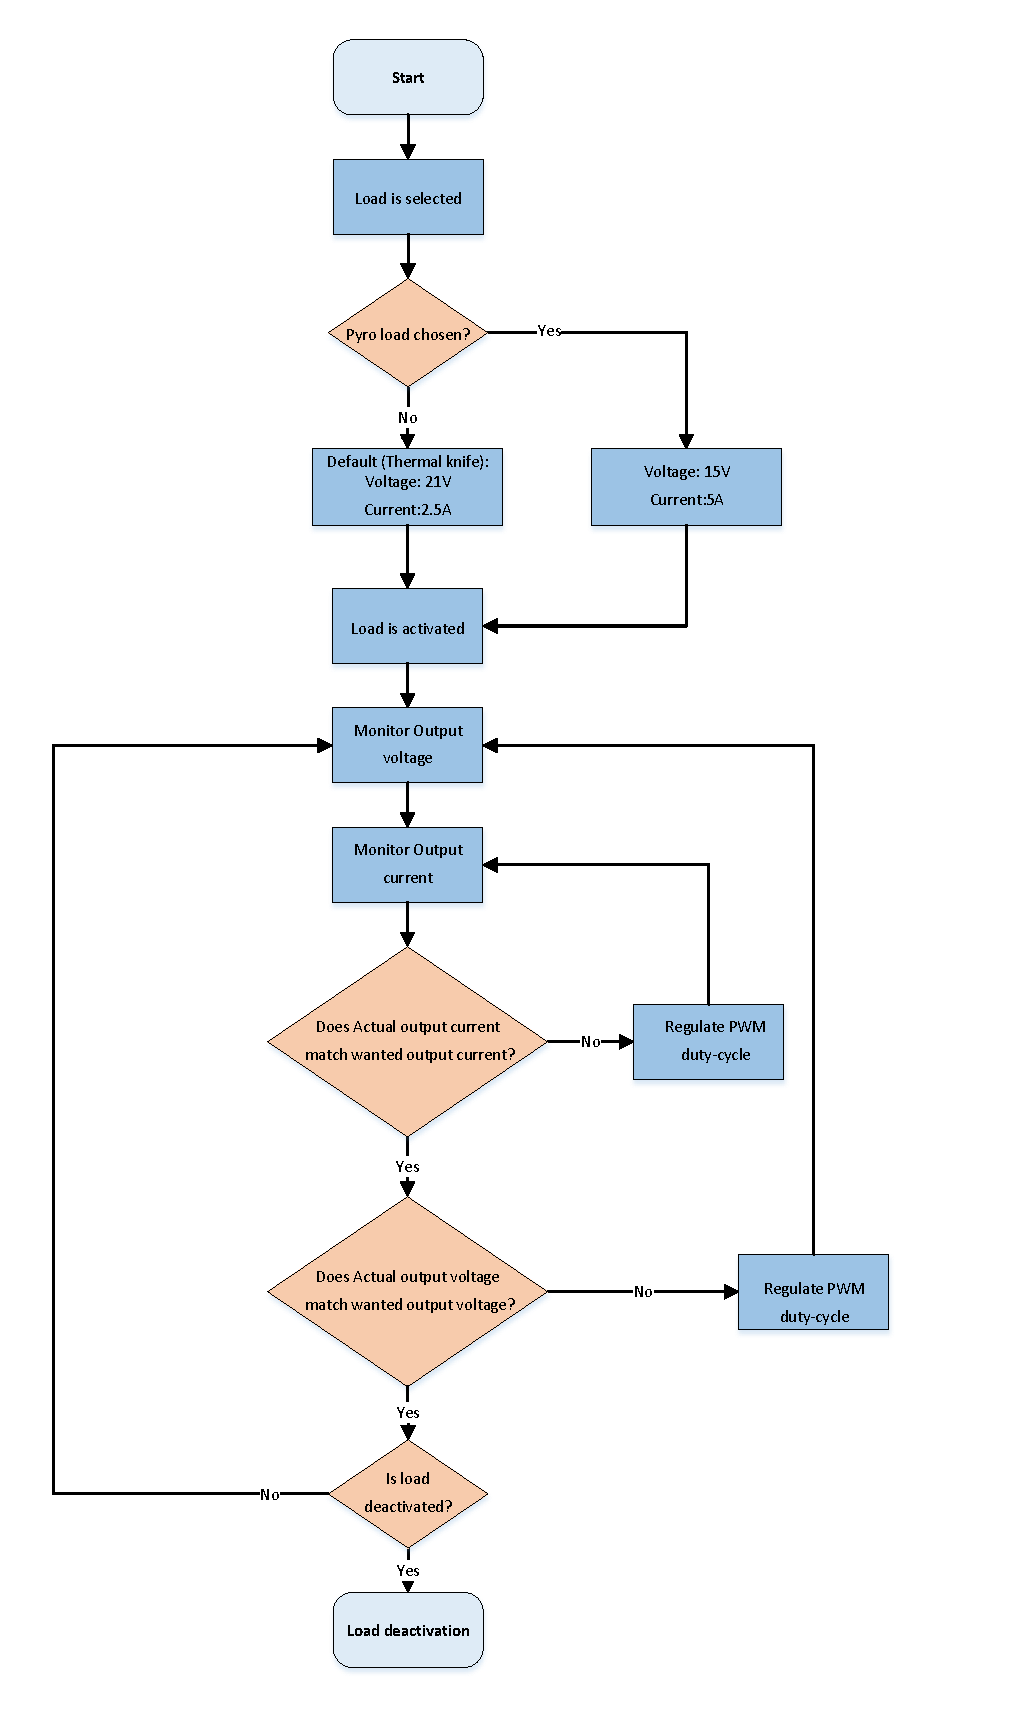
\includegraphics[width=0.7\linewidth]{../Dokumentation/tex/kravspecifikation/billeder/Flow_diagram.pdf}
	\caption{Flowdiagram for Universal Actuator Drive}
	\label{fig:flowdiagram}
\end{figure}
	
	
\chapter{Projektafgrænsning}
I dette afsnit er der beskrevet en afgrænsning af projektets indhold. Her er der taget udgangspunkt i det den ønskede funktionalitet af produktet, som sammenholdes med den egentlige opnåede funktionalitet. Elementer af projektet der er specificeret, men ikke implementeret er angivet i dette afsnit og uddybet i afsnit~\ref{future}. 

Produktets kernefunktionaliteter er prioriteret under udviklingen. Her er især prioriteret efter elementer, som kræves funktionsdygtige, før andre elementer kan udvikles. Her er udviklet en base for produktet, hvorpå flere krav og funktionaliteter skal kunne påføres.

Der blev valgt, at tage udgangspunkt i en converter med en statisk udgang. Dette ville skabe et udgangspunkt, og genere en erfaring, der ville give base for en videreudvikling til en dynamisk udgang af converteren.  

Det er valgt, at vikling af transformatoren sker af gruppen selv. Dette vil give en erfaring inden for området, der giver indsigt i hvad der er realistisk at designe efter. Derudover vil det også give et indblik i problematikkerne i vikling af en transformator. 

Converteren er designet efter de termiske krav, ved løbende vurdering og optimering af effekttabet i komponenterne.

Ved udvikling af elektroniske produkter til rumfart, kræves det udviklet med EEE-komponenter. Disse er meget omkostningsfulde, og er derfor ikke blevet brugt i projektet. Til gengælde er der brugt Terma-godkendte komponenter. Med disse komponenter har Terma en erfaring med, at opsætte disse til EEE-komponenter.  

Det blev specificeret at converteren skulle kunne operere ved et specifikt temperaturinterval. Det blev sikret ved kontrol af komponenternes specifikationer.

For at sikre en stabil indgangsspænding på converteren er det nødvendigt at implementere et indgangsfilter. Dette filter er blevet stillet tilrådighed af Terma, da det blev besluttet at fokusere andetsteds. Dette filter vil ikke blive beskrevet i denne rapport, men funktionaliteten af det er beskrevet i dokumentationen.

\fxnote{Beskriv PWM-forsyning}




	
	\chapter{Metode og proces}

\section{Metoder}

\subsection{ASE-modellen}
Til dette projekt er der brugt en iterativ udviklingsproces. Det er gjort da en iterativ proces er særligt velegnet til projekter, hvor kendskabet til domænet kan være begrænset. 

Der er taget udgangspunkt i den generelle ASE udviklingsmodel~\cite{udviklingsproces}, med den iterative proces trukket indover, hvilket ses på figur~\ref{fig:ASE}.
\begin{figure}[H]
	\center
	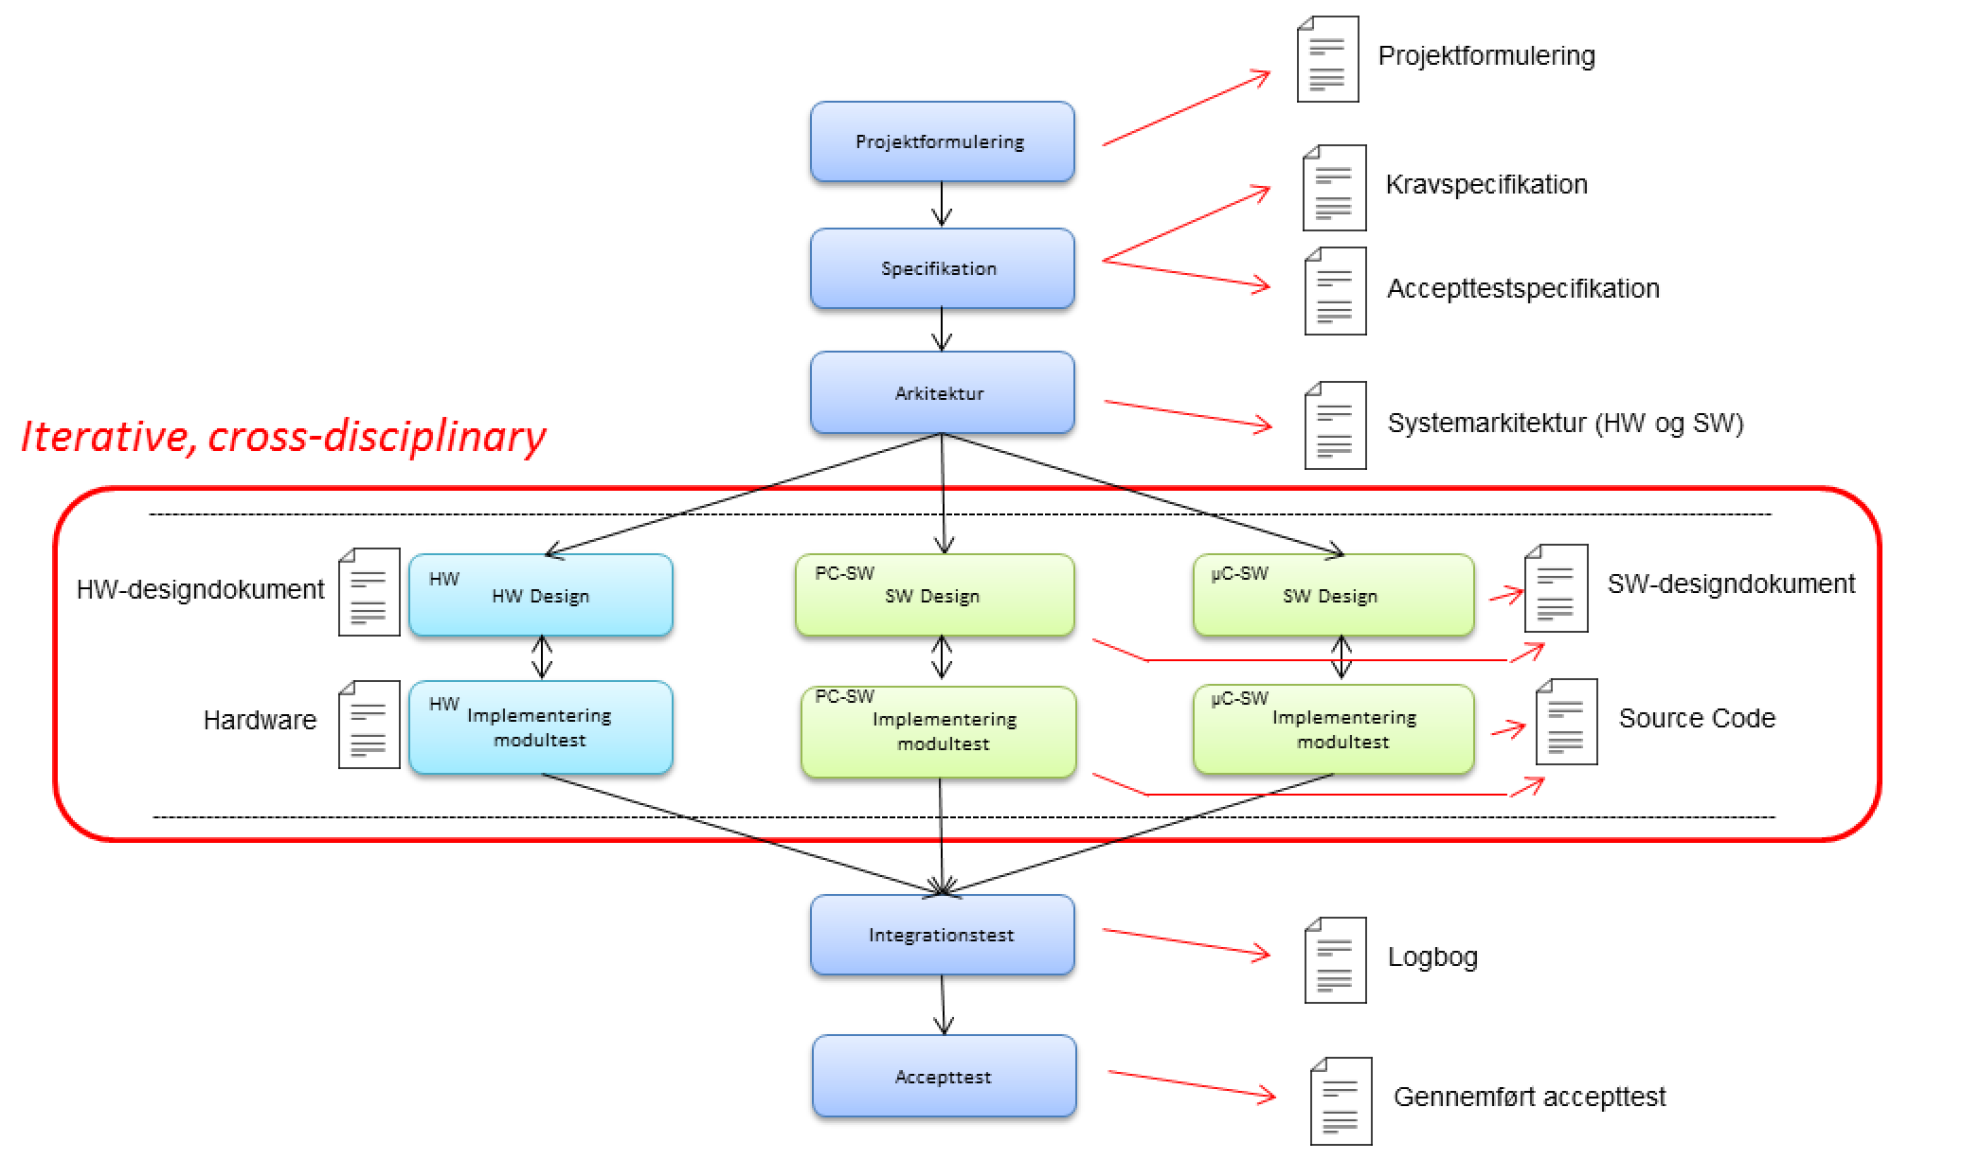
\includegraphics[max width=0.7\linewidth]{/tex/Metodeproces/billeder/ASEmodel.png}
	\caption{ASE model med fokus på iterativ proces}
	\label{fig:ASE}
\end{figure}  
I begyndelsen hvor produktet bliver specificeret med krav, har det ikke været så iterativt som de efterfølgende faser. Det skyldes at oplægget er kommet fra Terma, som har været med til at specificere kravene, og de har derfor ligget forholdsvis fast. Der har været få ændringer løbende, men det er begrænset.

Til gengæld har især design-, implementerings- og testfasen fungeret iterativt. Her er produktet blevet forbedret i små bider. Inden hver iteration begyndes gøres det klart, hvad der skal ske og hvad der skal opfyldes, inden næste iteration kan påbegyndes. 

\subsection{SysML}
Til at udarbejde systemarkitektur og design af systemet er der benyttet SysML. De anvendte SysML metoder for projektet har været block definitions diagrammer (BDD) og interne blok diagrammer (IBD). BDD'et er brugt til at nedbryde systemerne i mindre blokke, som dermed skal give et bedre overblik over systemets dele, og funktionen af disse. IBD'et viser den hardwaremæssige sammenhæng blokkene imellem.    

Ved at bruge er det nemmere for andre udviklere at sætte sig ind i systemet, og samtidig gør det designfasen nemmere, når systemets virkemåde er fastlagt forinden.

\subsection{UML}
Ofte benyttes UML mest til analyse og udarbejdelse af softwarearkitekturen. I dette projekt er UML metoden flowdiagram istedet brugt til at give et overblik over systemets ønskede virkemåde. Flow diagrammer giver et overblik over de valg, systemet gennemgår når det er aktivt.   

\subsection{MoSCoW} 
MoSCoW er en måde at prioritere krav på, alt efter hvor vigtige de er for det samlede produkt.  
De stilles op i "must", som er krav der skal overholdes. Næste prioritering er "should", som er krav der burde være overholdt. "Could" er features der ville være gode til produktet, men som der ikke forventes at være tid til at implementere. Sidste prioritering er "won't", hvilket er features som produktet ikke vil have. Med prioriteringen bør "must" kravene være opfyldt inden der kigges på "should" kravene. 

\section{Proces}
Som beskrevet tidligere har udviklingsprocessen fungeret iterativt. Til at implementere udviklingsmodellen, er der brugt Scrum~\cite{Scrum}. Scrum er valgt, da det er et projektsstyringsværktøj, begge medlemmer har haft stor succes med at bruge i tidligere semesterprojekter. Med en gruppe på to, er det ikke alle dele fra Scrum, som giver mening at bruge. Til dette projekt har det især været benyttet i forbindelse med daglige Scrum møder, og taskboards med backlog items. 

Til de daglige møder tages arbejdet fra dagen før op. Her forklares det, om man har været i stand til at udføre sine opgaver, og hvis ikke, hvilke problematikker det skyldes. Yderligere planlægges det, hvad der skal ske til næste gang. De daglige møder sørger for, at der bliver reflekteret over arbejdet løbende, hvilket sørger for at valgene der tages er gennemtænkt. 

Hver fase fra ASE modellen er blevet anset som iterationer, og har fået et taskboard hver. Hver enkelt iteration er delt op i mindre opgaver, der er lagt ind som backlog items på deres respektive taskboards. Design, implementerings og test iterationen er yderligere delt op i 3 faser for at bevare overblikket. På figur~\ref{fig:Taskboard} ses et øjebliksbillede af taskboardet for 3. iteration af design, implementerings og test.
\begin{figure}[H]
	\center
	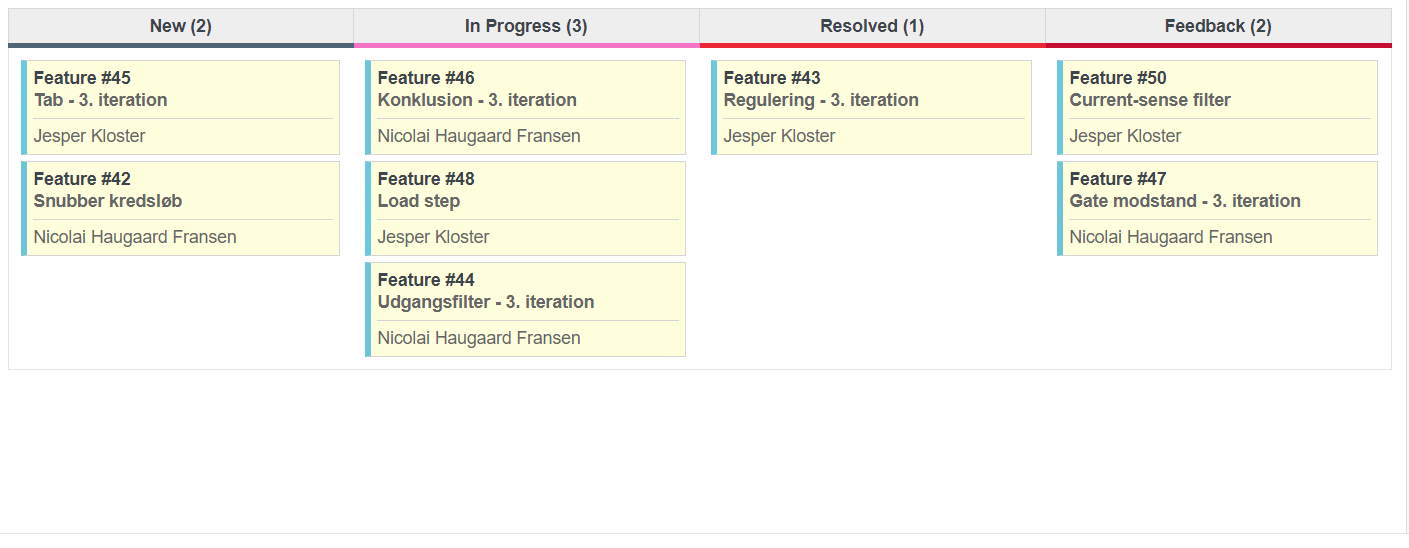
\includegraphics[max width=1\linewidth]{/tex/Metodeproces/Billeder/Scrumtask.png}
	\caption{Scrum taskboard}
	\label{fig:Taskboard}
\end{figure}        
Taskboardet sørger for at give et overblik over hvilke opgaver, der er påbegyndt og hvilke der mangles at blive lavet. På denne måde sikres det, at der ikke sidder to med samme opgave, og der er ikke opgaver, som bliver forsømt.

Til konfigurationsstyring er der benyttet et repository over Github~\cite{Github}. Det er brugt til deling af dokumenter og versionshistorik af disse. Yderligere er rapport, dokumentation og procesbeskrivelse skrevet i programmet LaTeX~\cite{Latex}. Kombinationen mellem LaTeX og Github gør det nemt at merge ændringer i dokumenterne. Det giver mulighed for at ændre i dokumenterne samtidigt, uden det skaber problemer. Samtlige dokumenter og bilag, som er vedlagt, har være administreret over Github.
Den interne kommunikation i gruppen er foregået over facebook. Det omhandler mødetidspunkter, spørgsmål og generelle informationer. Den eksterne kommunikation med vejleder og kontaktpersoner fra Terma er foregået over mail.  

Der har i projektperioden været afholdt 3 forskellige slags møder. De interne daglige møder, vejledermøde med Arne Justesen og eksterne møder med kontaktpersonerne fra Terma, Johnny Laursen og Hans Jensen. 

Langt hen ad vejen har der været afholdt vejledermøder en gang i ugen. Her har der på forhånd været tilsendt en dagsorden til vejlederen. Til møderne har der været en referent og en mødeleder, der sikrer, at dagsordenen overholdes. Disse roller er gået på skift fra møde til møde. Møderne har været brugt til, at diskutere arbejdet fra den forgangne uge og eventuelle opståede problemer. Derudover en forventning om opgaver der skal udføres inden næste møde. De omdiskuterede problemer har både været faglige- og rapportmæssige. 

Der har været afholdt møder med kontaktpersonerne fra Terma næsten hver uge. Igen har der været sendt information til kontaktpersonerne forinden, for at give et overblik om hvad der skal diskuteres. Ved disse møder har der været god mulighed for, at diskutere de fagligt opståede udfordringer, er opstået undervejs. Det er også her eventuelle ændringer af krav til produktet har været diskuteret. Under design-, implementerings- og testfasen har der dagligt været faglige diskussioner. Det har været yderst produktivt, at kunne løse et eventuelt problem med det samme, istedet for at vente til næste ugentlige møde. 

For yderligere information om den procesmæssige del af projektet henvises til dokumentet "Procesbeskrivelse" i bilagsmappen.  
	
	
\chapter{Analyse}
I dette afsnit beskrives de betragtninger og valg, der er blevet foretaget i løbet af produktudviklingen. Der er blevet vurderet på hvilke elementer der er nødvendige for realisering af produktet. Ved hvert af disse elementer er der foretaget en vurdering af hvilke muligheder og alternativer elementerne har. Der er også foretaget et vurdering på fordele og ulemper samtlige alternativer, der er blevet undersøgt i projektet. Ud fra disse vurderinger er der valget af de brugte teknologier blevet foretaget. 

\section{Converter topologi}
Converter topologien er en essentiel del af converterens endelige funktionalitet. Derfor er der undersøgt fordele og ulemper ved flere forskellige converter topologier. Converteren skal kunne konvertere indgangsspændingen til en mindre udgangsspænding, derfor er der udelukkende undersøgt topologier med denne funktionalitet. De undersøgte topologier er buck converteren, push-pull converteren og flyback converteren, som kan drives i både CCM og DCM. Disse convertere er yderligere beskrevet i dokumentationens afsnit 4.

\subsection{Buck converter}
Buck converteren er en af mere simple converter topologier, da den består af relativt få komponenter. sammen med dette er en af fordelene ved en buck converter, at der altid vil løbe en strøm i spolen. Det vil genere en minimal ripple-spænding på udganen, og derfor også et lille tab i udgangsfilteret. 

En stor ulempe ved buck converteren er at switch-komponenten, ofte en MOSFET, er placeret i den positive forsyningslinje. Det giver komplikationer ift. at drive MOSFET'en. Det vil kræve flere komponenter, og derfor også et mere kompliceret kredsløb. Af denne grund er buck converteren blevet fravalgt\cite{buck-converter}.

\subsection{Push-pull converter}

\subsection{Flyback converter}
Flyback converteren er en videreudvikling af buck converteren. Det er en transformator baseret topologi, som derfor giver et ekstra mulighed for effektoverførsel. Transformatoren erstatter spolen i buck converteren og derfor består de af det samme antal komponenter. Transformatoren giver desuden muligheden for sikre galvanisk adskillelse mellem indgangen og udgangen. 

En ulempe ved flyback converteren er en diskontinuert strømform i transformatoren, da der ikke løber strøm primær- og sekundærviklingen på samme tid. Det vil skabe større ripple- og RMS-strømme, og derved også genere et større tab i komponenterne\cite{SMPS-topologies}. 

En flyback converter kan drives på to overordnede måder - CCM og DCM. De to metoder bidrager yderligere med hver deres fordele og ulemper, som også vil blive beskrevet. 

Forskellen på de to metoder ligger i kurveformen for den strøm der løber i transformatorviklingerne. Ved CCM vil der altid løbe en strøm i enten den ene, eller den anden vikling. I modsætning til DCM hvor strømmen vil have en dødtid i løbet af en switch-periode. For at DCM skal kunne opretholde den samme udgangsstrøm som CCM, vil det betyde at peak- og RMS-strømmene ved DCM bliver større. Det giver derved anledning til et større effekttab. 

Fordelen ved at operere i DCM er primært en simplificering af reguleringssløjfen. CCM indeholder et dominerende nulpunkt langt nede i frekvens, der kan gøre systemet ustabilt, hvis der ikke tages højde for dette. Nulpunktet begrænser samtidig båndbredden, og dermed også systemets responstid. 

Ud fra disse undersøgelser er det blevet valgt, at arbejde videre med en flyback converter opereret i CCM. Dette vil sikre en converter hvor det er muligt, at holde effekttabet og kompleksiteten i converteren på et acceptabelt niveau. 

\section{Reguleringsmetode}
Der er to overordnede reguleringsmetoder der bruges til regulering i en DC/DC converter - Spændingsregulering og strømregulering. Ved spændingsregulering vil reguleringen udelukkende ske på baggrund af et spændingsfeedback til reguleringssløjfen. Ved strømregulering, reguleres der både efter strømmen og spændingen på udgangen. Det sikre en overstrømsbeskyttelse for converteren. Den ekstra reguleringsløkke vil samtidig simplificere reguleringen af en flyback converter i CCM. 

\noindent Derfor vælges det, at implementere en strømregulering i converteren. 

\section{PWM-controller}
PWM-controlleren er en central del af en DC/DC converter. Det er denne controller der står for at generere switch-signalet til converterens switch-element. Af denne grund er der mange krav PWM-controlleren skal leve op til. Den skal først og fremmest understøtte den valgt reguleringsmetode. Den skal kunne generere den maksimale duty-cycle der vil kunne fremstå i converterens switch-signal. Den skal kunne opretholde den valgte switch-frekvens. Derudover skal den også kunne generere et switch-signal med en amplitude der er høj nok, til at kunne drive den valgte MOSFET.

Ud fra disse krav, er det valgt at bruge en PWM-controller af typen UCC1801\cite{UCC1801}. Denne controller lever op til de førnævnte krav, og desuden understøtter den peak-current regulering. Den har indbyggede reguleringssløjfer, således nødvendigheden for eksterne komponenter mindskes. Derudover indeholder den flere sikkerhedsfunktioner ved opstart. Det er også en controller Terma har erfaringer med, og ved den kan omsættes til en lignende komponent der er godkendt til rumfart. 

\section{Transformator} \label{Transana}
Størrelsen på transformatoren betyder meget ift. temperaturstigningen, som en konsekvens af effektafsættelsen i transformatoren. Den termiske modstand i den er afhængig af størrelsen\cite{epcos-cores}. Derfor er det valgt at bruge en RM8\cite{RM8} som er den største kerne, der stadig overholder kravene for dimensionerne. Desuden er kernetypen RM blevet anbefalet af Terma, der har haft god erfaring med brug af disse i lignende konfigurationer. Der er valgt at bruge kernematerialet 3f3\cite{3f3}, da Terma har mere præcise målinger af materialets specifikationer, ift. databladets tolerancer.


	
	
\chapter{Systemarkitektur}
I det følgende afsnit beskrives systemarkitekturen, der er blevet udarbejdet i løbet af projektet. Projektet indeholder udelukkende hardware, derfor er der kun blevet udarbejdet arkitektur for dette. Arkitekturen ligger til grundlag for designprocessen i det videre projektforløb. Systemarkitekturen er overordnet beskrevet i det følgende afsnit, og uddybet i dokumentationens afsnit 3.

Hardwarearkitekturen er blevet beskrevet ved SysML's BDD og IBD. Der er blevet udarbejdet overordnede diagrammer for systemet, der skal give et overblik over det samlede system.

\section{Block Definition Diagram}
Figur~\ref{fig:BDD} viser et BDD for det samlede system. Det giver et overblik over de dele systemet indeholder, og hvilke forbindelser hver blok skal indeholde. 

\begin{figure}[H]
	\centering
	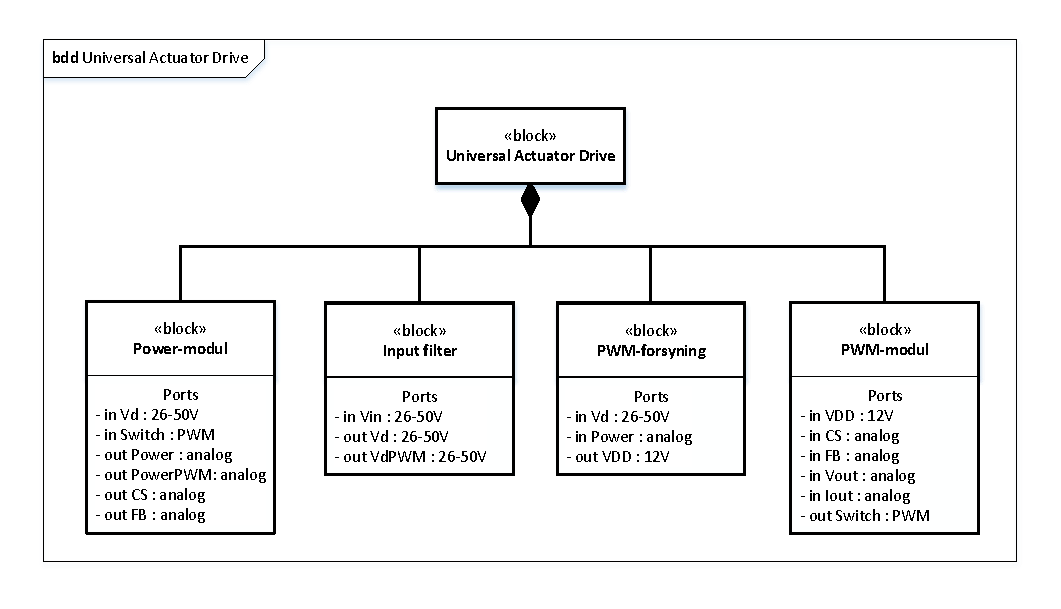
\includegraphics[width=1\linewidth]{../Dokumentation/tex/systemarkitektur/billeder/BDD.pdf}
	\caption{BDD for det overordnede system}
	\label{fig:BDD}
\end{figure}

\noindent Universal Actuator Drive består af fire overordnede blokke - et Power-modul, et Input-filter, en PWM-forsyning og et PWM-modul. Power-modulet indebærer selve effektoverførelsen fra indgang til udgang. Det er i dette modul de dominerende effektafsættelser sker, og derfor også her det termiske design skal optimeres. 

Input-filteret indebærer det filter der sikre en stabil indgangsspænding til Power-modulet. Derudover skal det fjerne højfrekvent ripple-spændinger fra indgangssignalet. 

\noindent PWM-forsyningen indebærer en regulator til regulering af PWM-modulets forsyningsspænding. Her vil der udvikles en metode der forsyner regulatoren fra indgangskilden under opstart, og udgangen når denne er stabil.

PWM-modulet indebærer PWM-controlleren der skal regulere udgangen til den ønskede belastning. Dette sker ved tilpasning af switch-signalet, samt strøm- og spændingsregulering af udgangen.

\section{Internal Block Diagram}
Figur~\ref{fig:IBD} viser et IBD for det samlede system. Det er blevet udarbejdet ud fra systemets BDD. IBD'et giver et overblik forbindelserne internt i systemet. Det viser også hvilke forbindelser systemet modtager fra andre systemer, altså grænsefladerne til omverdenen. Kravene for disse forbindelser er nærmere beskrevet i dokumentationens afsnit 3.2.

\begin{figure}[H]
	\centering
	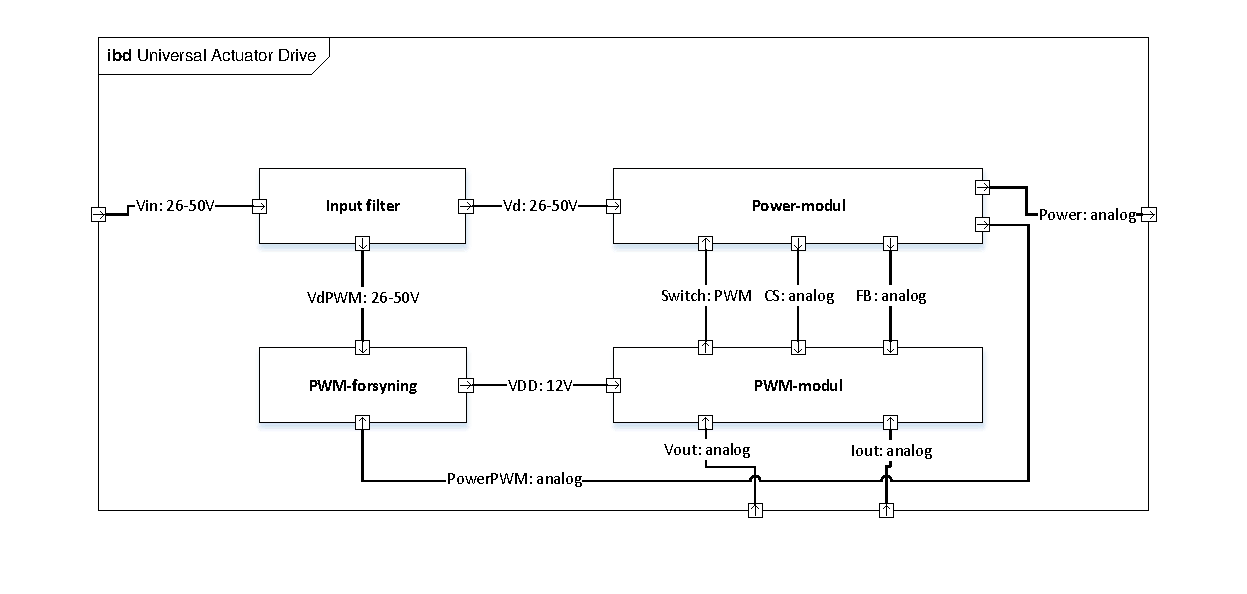
\includegraphics[width=1\linewidth]{../Dokumentation/tex/systemarkitektur/billeder/IBD.pdf}
	\caption{IBD for det overordnede system}
	\label{fig:IBD}
\end{figure}
	
	\chapter{Design, implementering og test}
I det følgende afsnit vil der blive gjort redde for designprocessen i projektforløbet. Her vil de meste essentielle dele for produktet blive beskrevet, mens en yderligere beskrivelse kan findes i dokumentationens afsnit 4-6.

Designprocessen blev delt op i tre overordnede iteration. I det følgende afsnit vil det derfor tydeliggøres, hvad der blev designet i den gældende iteration. 


\section{Første iteration}
Målet med 1. iteration var undersøgelse og valg af converter topologi. Herefter blev der opstillet en ideel simuleringsmodel for converteren, således analyse og simulering kunne sammenholdes. 
Kravet for at gå videre til 2. iteration, var opnåelse af en simulering der stemte overens med teorien. 



\subsection{Flyback converter - CCM}
Der blev valgt en flyback converter opereret i CCM, som converter topologi i projektet. En sådan converter deles op i en primær- og en sekundær side. Primærsiden består af transformatorens primærvikling og et switch-element, der typisk er en MOSFET. Sekundærsiden består af transformatorens sekundærvikling en diode, en kondensator og udgangsbelastningen. En oversigt over den ideelle flyback converter er vist på figur~\ref{fig:flyabck_ideal}. 

\begin{figure}[H]
	\centering
	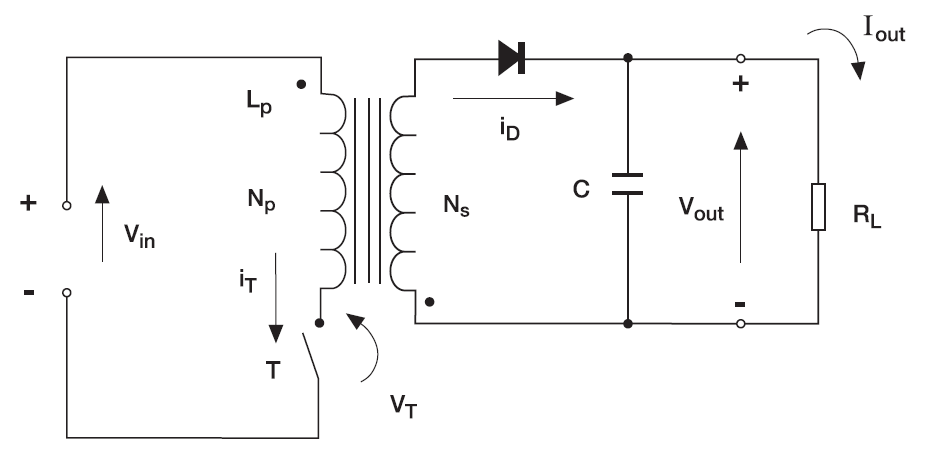
\includegraphics[width=0.7\linewidth]{../Dokumentation/tex/1iteration/billeder/flyback_ideal.png}
	\caption{Ideelt diagram for flyback converteren
		\cite{SMPS-topologies}}
	\label{fig:flyabck_ideal}
\end{figure}

Når MOSFET'en er ON, vil der være en positiv spænding over primærviklingen ved prikenden af viklingen, der er lig indgangsspændingen. Da denne spænding er positiv, vil det få strømmen i viklingen til at stige lineært over den tid MOSFET'en er ON. Strømændringen er bestemt ud fra formlen:
\begin{equation}
V = L \cdot \frac{di}{dt}
\end{equation}

Fordi polariteten af sekundærviklingen er modsat primærviklingen, vil dioden være forspændt i spærreretningen da kondensatoren vil opretholde udgangsspændingen over belastningen. Når dioden ikke kan lede strømmen fra sekundærviklingen, vil transformatoren oplagre energi i kernen når MOSFET'en er ON. Når MOSFET'en går OFF vil strømmen i viklingen ikke kunne skifte momentant. Det vil vende polariteten af transformatoren, så der nu er en positiv spænding diode enden af sekundærviklingen. Nu vil dioden være forspændt i lederetningen, og derfor lede den energi der er blevet oplagret i kernen, i form af en strøm. Den strøm vil nu holde den ønskede udgang, men også oplade kondensatoren, således den kan opretholde udgangsspændingen i næste ON-periode. Da der nu vil være en negativ spænding over sekundærviklingen ift. prikenden af den, vil strømmen i viklingen aftage i løbet af MOSFET'ens OFF periode på baggrund af den førnævnte formel. 

Kurveformen for strømmene i en flyback transformator er vist på figur~\ref{fig:flyabck_ideal_currents}. Her ses det der blev forklaret før. Når MOSFET'en er ON, vil strømmen i primærviklingen rampe op, mens strømmen i sekundærviklingen er 0. Når MOSFET'en er OFF vil strømmen i sekundærviklingen rampe ned fra det niveau primærstrømmen nåede, mens strømmen i primærviklingen nu vil være 0. Niveau-forholdet mellem strømmene i viklingerne, vil blive bestemt af viklingsforholdet i transformatoren. Skal converteren bruges til omsætning af store spændingsændringer fra indgang til udgang, kan dette bruges for at mindske tabet. 

\begin{figure}[H]
	\centering
	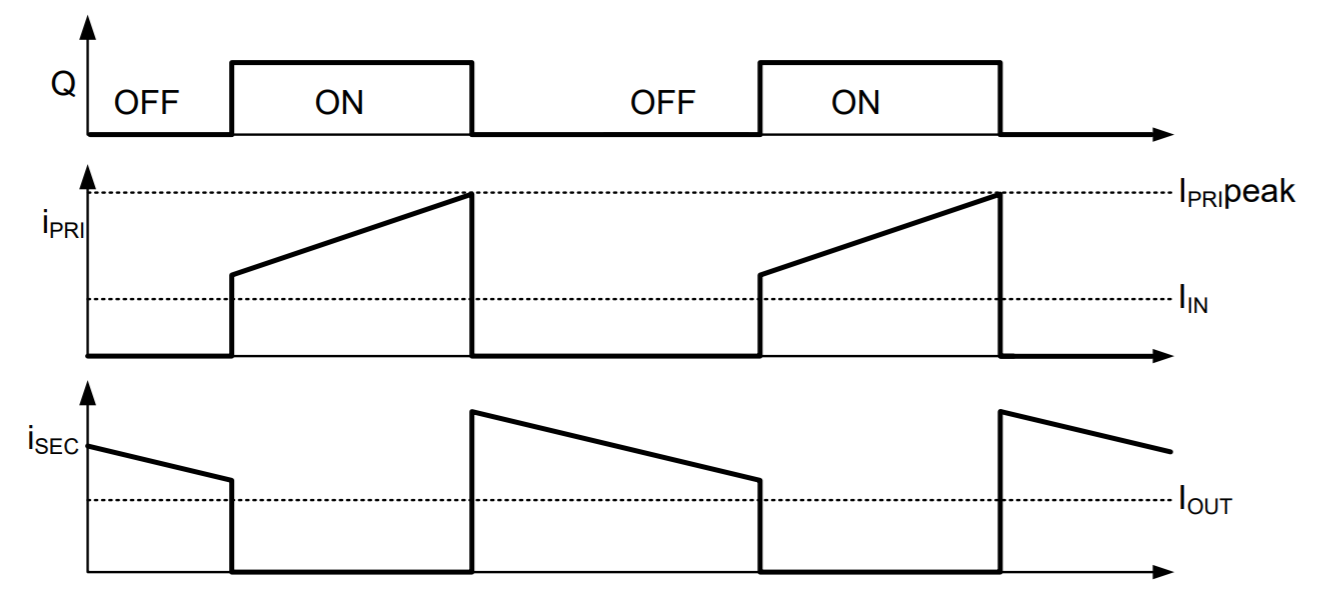
\includegraphics[width=0.7\linewidth]{../Dokumentation/tex/1iteration/billeder/CCM_transformer_current.png}
	\caption{CCM transformator strømme}
	\label{fig:flyabck_ideal_currents}
\end{figure}

selvom transformatoren i helhed opererer i CCM, vil strømmene i individuelt i viklingerne være diskontinuerte. Det betyder peak-strømmene i viklingerne bliver større for at kunne opretholde den ønskede udgangsstrøm. 

\noindent Overføringsfunktionen for flyback converteren i CCM er\cite{SMPS-topologies2}:
\begin{equation*}
	V_{out} = \frac{N_s}{N_p} \cdot \frac{D}{1-D} \cdot V_{in}
\end{equation*}

Da den mindste indgangsspænding og største udgangsspænding converteren skal designes efter næsten er ens, vælges det at tage udgangspunkt i en transformator en et viklingsforhold på 1. Ud fra dette, og intervallet på indgangsspændingen på $26-50V$, kan den maksimale duty-cycle regnes til $D_{maks} = 0.447$ eller $44.7\percent$, og den minimale duty-cycle renes til $0.296$ eller $29.6\percent$.  

Selvinduktionen i transformatorviklingerne bestemmes ud fra den ønskede ripple-strøm i transformatoren og den valgte switch-frekvens. Der er valgt at tage udgangspunkt i en switch-frekvens på $100k\hertz$. Når der er valgt at have et omsætningsforhold på 1, vil denne selvinduktion være gældende for begge viklinger. Selvinduktionen i transformatoren kan designes ud fra følgende formel\cite{flyback-formler}:
\begin{equation*}
	L = \frac{V_{inmin} \cdot D_{min}}{I_{ripple} \cdot f_s}
\end{equation*}

RMS-strømmene i viklingerne har stor betydning for det endelige tab i converteren. Derfor estimeres de i den indledende fase, for at vurdere betydningen af dette. RMS-strømmen i primærviklingen regnes til $3.02A$, og RMS-strømmen i sekundærviklingen regnes til $3.36A$. Begge er regnet ved en indgangsspænding på $26V$. 

Den ideelle converter er simuleret, for kontrol af dens funktionalitet. Figur~\ref{fig:flyabck_ideal_diagram} viser diagrammet for den ideelle converter. Her er der udelukkende fokuseret på transformatoren. Desuden er der indsat en kondensator på $223\micro F$, for at mindske ripple-spændingen på udgangen. Udgangen er blevet simuleret til det forventede $21V$ og $2.5A$, mens RMS-strømmene i transformatorviklingerne stemte overens med det beregnede. 

\begin{figure}[H]
	\centering
	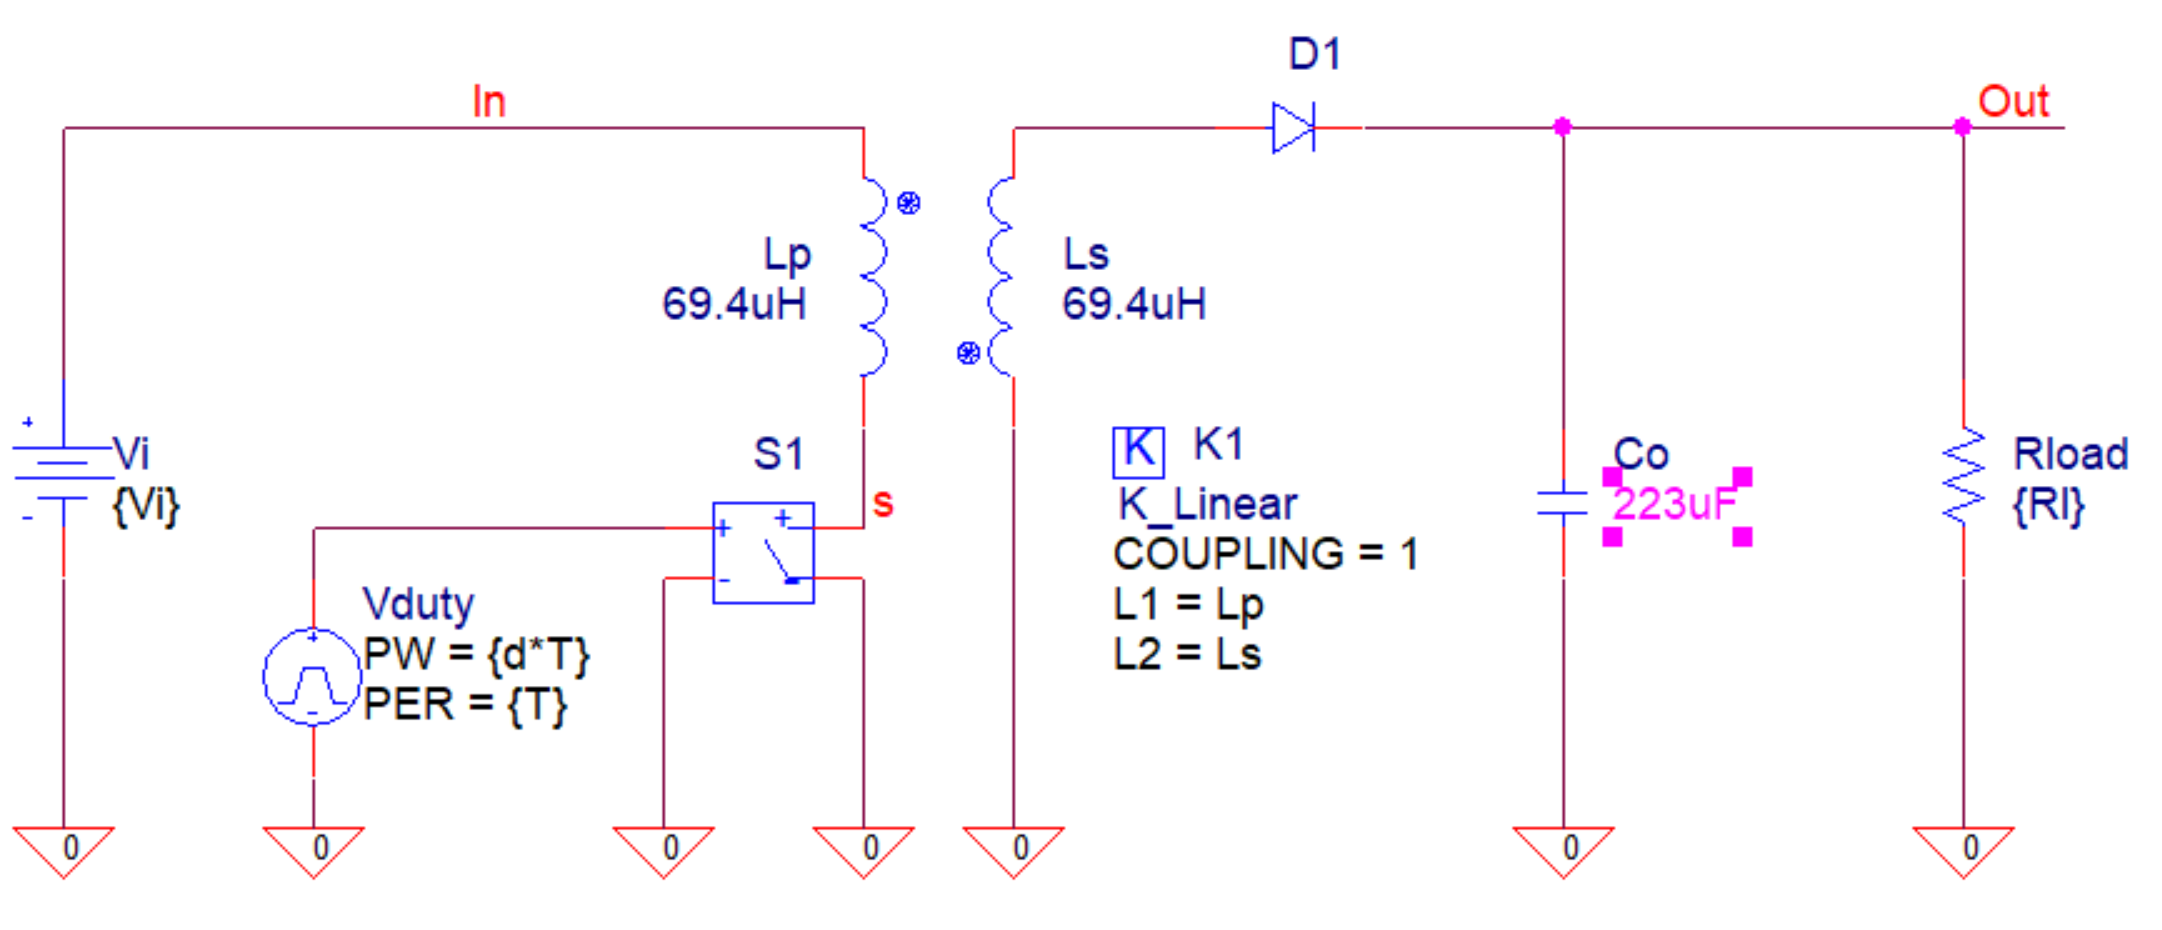
\includegraphics[width=0.7\linewidth]{../Dokumentation/tex/1iteration/billeder/flyback_ideal_diagram.png}
	\caption{Simulering af ideel flyback converter}
	\label{fig:flyabck_ideal_diagram}
\end{figure}

\noindent De præcise beregninger og simuleringer er beskrevet i dokumentationens afsnit 4.4.










\section{Anden iteration}
Målet for 2. iteration var, at indsætte ikke-ideele komponenter ind i modellen fra første iteration. Herudover skulle modellen implementeres for første gang. 
Kravet for at gå videre til 3. iteration var en funktionsdygtig implementeret converter. 
I dette afsnit beskrives hvordan nøglekomponenterne i konverteren er designet, og første implementering af converteren.

\subsection{Transformator}
Flyback converteren fungerer transformatoren lidt anderledes, i forhold til mange andre konstruktioner. Normalt vil der løbe en strøm i både den primære og sekundære vikling på samme tid. På den måde kan energien i transformatoren transformeres direkte fra den primære vikling til den sekundære vikling. Dette er ikke muligt i denne converter typologi, da der kun vil løbe strøm i én vikling ad gangen. Den energi, der skabes i den primære vikling, skal derfor kunne opbevares, indtil der begynder at løbe en strøm i sekundærviklingen. Sker det ikke, går kernen i mætning, hvilket vil sige, at der ikke er en lineær sammenhæng imellem transformatorens H-felt og B-felt.
Dette sikres ved, at indsætte et luftgab i kernen, som øger den magnetiske modstand. Det gør, at kernen kan opbevare mere energi.

I 1. iteration blev det valgt at tage udgangspunkt i en 1:1 transformator. Desuden er det i 2. iteration vigtigst, at få en velfungerende transformator. Derefter kan der senere optimeres på et mere optimalt viklingsforhold, hvis det vurderes nødvendigt. 

Med den estimerede nødvendige induktans beregnet i 1. iteration til $69.43\micro H$, blev energien, der induceres i primærviklingen udregnet til \begin{equation} \label{Primary_energy}
E = \frac{1} {2} \cdot L \cdot {I_{pk}}^2 = 1.083\milli J
\end{equation}

Denne energi skal kunne opbevares i kernen, for at undgå den føromtalte mætning. Hvornår en specifik transformator går i mætning afhænger af selve kernen og dets kernemateriale. Her faldt valget på en RM8 kerne og materialet 3f3, hvilket der er argumenteret for i sektion~\ref{Transana}.
På baggrund af databladet for 3f3, blev luftgabet designet efter at have et maksimalt B felt på $250mT$. Det gav et nødvendigt luftgap på:
\begin{equation} \label{Airgap}
l_g = \frac{L \cdot {I_{pk}}^2 \cdot \micro_0}{B^2 \cdot A_0} = 690.98\micro m
\end{equation}

Dette gav en fornyet induktans på $49\micro H$. Herefter bruges $A_L$ for 3f3 materialet og induktansen til at beregne vindingstallet, som blev udregnet og afrundet til 18 vindinger.
Analysen er herefter holdt op imod simuleringen i p-spice, at sikre at analyse og simulering stemmer overens.
 
Viklingen af transformatoren er sket med en kobbertråd med en diameter på $0.425mm$. Det er en tyndere tråd end analyseret, da der med den beregnede trådtykkelse på $0.45mm$ ikke i praksis kunne vikles 18 vindinger. Det har samtidig øget vindingstallet til 19, for stadig at udnytte hele kernens bredde bedst muligt. Med denne trådtykkelse og vindingstal er hele bredden af kernen på $8.6mm$ fuldt udnyttet. Igen for at fylde kernen ud, er der for både primær- og sekundærsiden viklet 3 viklinger i parallel, for at udnytte højden af kernen. Det giver samlet den tredobbelte højde med 6 viklinger i alt, hvilet ender i en højde $2.867mm$. Viklingen er udført ved skiftevis at vikle en primærvikling og en sekundærvikling. På den måde optimeres koblingen i transformatoren. Imellem viklingerne indsættes tape for at sikre det holdes stramt. På figur~\ref{fig: viklingsoverblik} vises et overblik over viklingerne og dimensionerne. 
\begin{figure}[H]
	\center
	\includegraphics[max width=0.7\linewidth]{../dokumentation/tex/2iteration/billeder/viklingsoverblik.png}
	\caption{Overblik over viklingsantal og tykkelse}
	\label{fig: viklingsoverblik}
\end{figure}
\noindent Med vindingstallet på 19 istedet for 18 er selvinduktionen og dermed strømmene i transformatoren igen korrigeret. Herunder ses den endelig analyserede selvinduktion, ripplestrøm og peakstrøm for den viklede transformator.
\begin{equation} \label{L_2}
L_2 = N^2 \cdot A_L = 57.76\micro H
\end{equation}
\begin{equation} \label{I_ripple_final}
I_{ripple} = \frac{V_{inmin} \cdot D_{max}}{L_2 \cdot f_s} = 2.01A
\end{equation}
\begin{equation} \label{I_pk_final}
I_{pk} = \frac{V_{out} \cdot I_{out}}{V_{inmin} \cdot D_{maks}} + \frac{I_{ripple}}{2} = 5.53A
\end{equation}
Den implementerede transformator ses på figur~\ref{fig: Viklettrans}
\begin{figure}[H]
	\center
	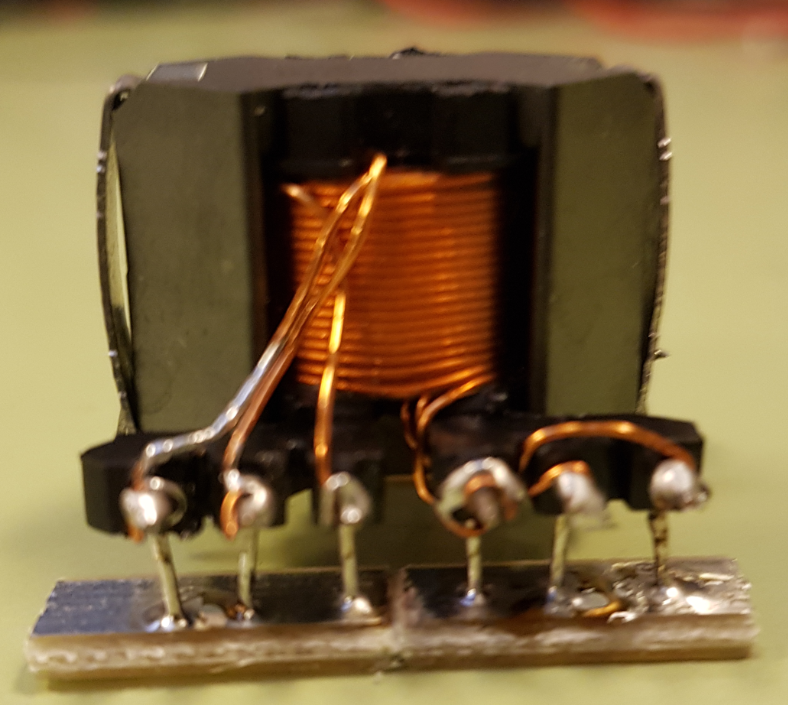
\includegraphics[max width=0.5\linewidth]{../dokumentation/tex/2iteration/billeder/Viklet_transformator.PNG}
	\caption{Viklet transformator}
	\label{fig: Viklettrans}
\end{figure}
\noindent Testen af transformatoren er udført ved at måle selvinduktionen i primær- og sekundærviklingerne samt spredningsselvinduktionen. Det er gjort med en impedansmåler. Her er der benyttet så korte ledninger som muligt samt 4-wire teknikken, for at undgå ekstra induktans fra ledningerne. 

For at måle selvinduktionen i primærviklingen måles henover primærviklingens to sider, mens sekundærviklingen holdes åben. Her laves et frekvenssweep fra $100Hz$ til $1MHz$. Samme fremgangsmåde for sekundærvikligen kan benyttes, men da transformatoren er 1:1, bør det være det samme.
Spredningsselvinduktionen er målt ved måle samme sted, henover primærviklingen, men derudover kortslutte sekundærviklingen. En ideel transformator vil give 0 i sådan en måling. Det betyder, at induktansen målt her, svarer til spredningsselvinduktionen. 

For yderligere forklaring af design, implementering og test af transformatoren henvises til dokumentationen afsnit 5.1, hvor dette er uddybet.

% Dokumentation af PWM-controller %
% UCC1801 %

\section{PWM-controller} \label{PWM}
PWM-controlleren er en vigtig del af en SMPS. Det er den der står for tilpasningen af switch-signalets duty-cycle, således udgangen holdes stabilt, når inputtet påvirkes eller ændres. Det er vigtigt at vælge PWM-controller ud fra kravene til converteren. PWM-controllere er ofte begrænset til en maksimal duty-cycle på enten $50\percent$ eller $100\percent$. Derudover skal der vælges, hvilken form for regulering af converterens udgangstrin der ønskes, da controlleren skal understøtte dette. 

Ud fra beregningerne af den maksimale duty-cycle i afsnit~\ref{maksimum_duty_cycle}, vælges det at PWM-controlleren maksimalt skal have en duty-cycle på $50\percent$. For at kunne opnå en mere præcis regulering, vælges det at bruge peak-current regulering. Denne form for regulering, regulerer efter peak-strømmen i transformatorens primærvikling. Da den regulere efter dette, opnås der også en strømbegrænser i regulerings-loopet. Ud fra disse krav vælges en PWM-controller af typen UCC1801\cite{UCC1801}. Det er en controller Terma har erfaring med, og derfor også nemt kan udskiftes med en space-godkendt controller.

\subsection{Funktionalitet}
På figur~\ref{fig:PWM_block_diagram} ses et funktionelt block diagram over UCC1801. Det indeholder controllerens overordnede komponenter, og giver et overblik over dens funktionalitet. 

\begin{figure}[H]
	\center
	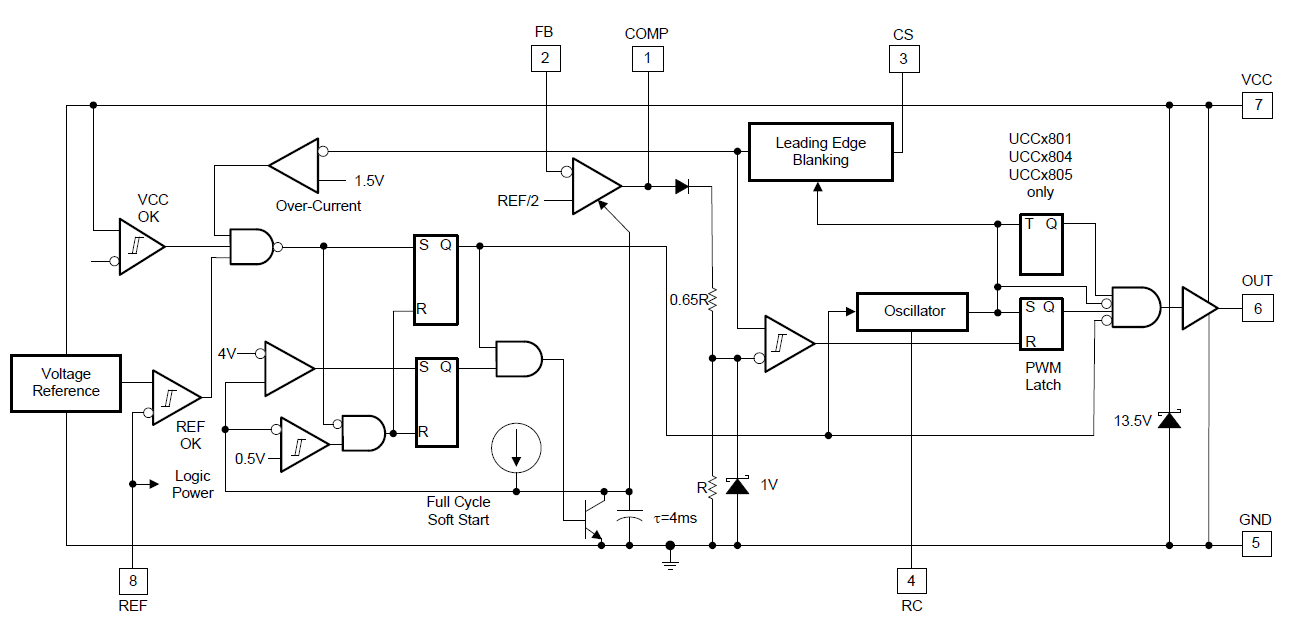
\includegraphics[max width=0.9\linewidth]{/tex/2iteration/billeder/PWM_block_diagram.PNG}
	\caption{UCC1801 - Funktionelt Block Diagram}
	\label{fig:PWM_block_diagram}
\end{figure}

Tabel~\ref{tab:ucc1801_specs} viser de mest essentielle specifikationer for UCC1801, i forhold til en flyback converter. Disse er udvalgte specifikationer fra databladet.

\begin{table}[H] 			
	\centering
	\begin{tabularx}{\textwidth}{|X|c|c|c|} 
		\hline
		\textbf{Specifikation} & \textbf{Min} & \textbf{Typ} & \textbf{Max} \\ \hline
		$V_{CC}$ &  &  & $12V$ \\ \hline
		$I_{out}$ &  &  & $1A$ \\ \hline
		$V_{Reference}$ & $4.925V$ & $5V$ & $5.075V$ \\ \hline
		$D_{max}$ & $48\percent$ & $49\percent$ & $50\percent$ \\ \hline
		$V_{on,th}$ & $8.6V$ & $9.4V$ & $10.2V$ \\ \hline
		$V_{off,th}$ & $6.8V$ & $7.4V$ & $8V$ \\ \hline
		Temperature Range & $-55\degreeCelsius$ &  & $125\degreeCelsius$ \\ \hline
		$f_{osc}$ & & & $1M\hertz$ \\ \hline
	\end{tabularx}

	\caption{Relevante specifikationer for UCC1801}
	\label{tab:ucc1801_specs}
\end{table}


\subsubsection{Ben konfiguration}
Der tages udgangspunkt i en UCC1801, med en PDIP pakke type. Figur~\ref{fig:ucc1801_pin_overview} viser en oversigt over ben konfigurationen for en sådan pakke. Det er en 8-bens IC, hvor samtlige ben bliver brugt. Benenes funktionalitet er overordnet beskrevet i tabel~\ref{tab:ucc1801_pin_functionality}, og vil blive uddybet i de følgende afsnit.

\begin{figure}[H]
	\center
	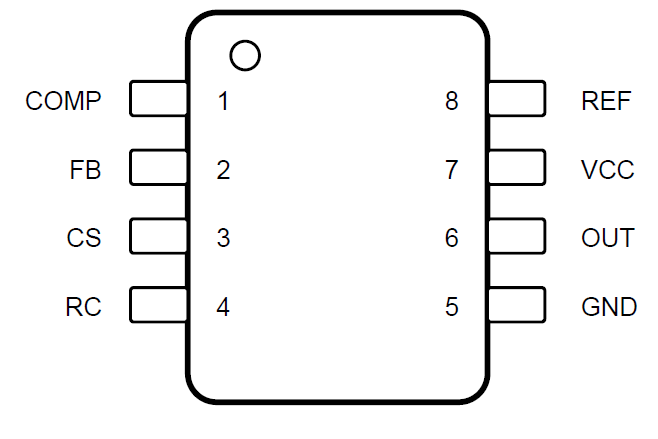
\includegraphics[max width=0.7\linewidth]{/tex/2iteration/billeder/ucc1801_pin_overview.PNG}
	\caption{Ben konfiguration for UCC1801}
	\label{fig:ucc1801_pin_overview}
\end{figure}

\begin{table}[H] 			
	\centering
	\begin{tabularx}{\textwidth}{|c|c|c|X|} 
		\hline
		\textbf{Navn} & \textbf{Ben} & \textbf{I/O} & \textbf{Beskrivelse} \\ \hline
		COMP & 1 & O & COMP er outputtet fra den indbyggede fejlforstærker. Dette ben bruges til at lave et feedback til FB benet i reguleringssløjfen. 	\\ \hline
		FB 	 & 2 & I & FB er inputtet til den indbyggede fejlforstærker. Den er forbundet til den inverterende indgang af forstærkeren. Den bruges sammen med COMP, som en del af reguleringssløjfen.\\ \hline
		CS   & 3 & I & CS er inputtet til current sense komparatorne. UCC1801 har to komparatorere til current sense: PWM komparatoren og overstrøms komparatoren. PWM-komparatoren bruges til, at trække udgangssignalet lavt, når CS-signalet overstiger $1V$. Overstrøms komparatoren er en indbygget overstrømsbeskyttelse. Den tvinger udgangen lav, så længe CS-signalet er over $1.5V$ \\ \hline
		RC 	 & 4 & I & RC er inputtet til oscillatoren. Oscillator frekvensen, og dermed også switch-frekvensen, sættes ud fra tidskonstanten mellem en modstand og en kondensator.  \\ \hline
		GND  & 5 & - & GND er ground for IC'ens komponenter.  \\ \hline
		OUT  & 6 & O & OUT er IC'ens output. Det er et PWM-signal, hvis duty-cycle afhænger af PWM-komparatoren. Outputtet skiftes mellem GND og VCC, hvilket betyder at VCC skal være høj nok, til at drive MOSFET'en.  \\ \hline
		VCC  & 7 & I & VCC er forsyning til IC'ens komponenter. Det foreslås at vælge en høj VCC, for at mindske støjpåvirkninger. For at mindske støj på forsyningen anbefales det, at bypasse VCC med en kondensator på minimum $1\micro \farad$, tæt på IC'en. \\ \hline
		REF  & 8 & O & REF er outputtet for IC'ens interne spændingsreference. Den bruges bl.a. som reference til fejlforstærkeren. Derudover forsyner den IC'ens logiske komponenter. For at mindske støj på referencen, anbefales det at bypasse REF med en kondensator på minimum $1\micro \farad$, tæt på IC'en. \\ \hline
	\end{tabularx}
	
	\caption{Ben funktionalitet for UCC1801}
	\label{tab:ucc1801_pin_functionality}
\end{table}

\subsection{Under Voltage LockOut}
UCC1801 indeholder en Under Voltage LockOut (UVLO) beskyttelse. Dette betyder at forsyningsspændingen skal være et bestemt niveau, før controlleren starter. Som en konsekvens af dette vil både outputtet og referencespændingen holdes lav, indtil grænseværdien er nået. For at have en hysteresemargin, har den både et turn ON og et turn OFF niveau. Ved UCC1801 er disse niveauer $V_{on,th}=9.4V$ og $V_{off,th}=7.4V$. Da amplituden af output-signalet er lig VCC, vil controlleren ikke prøve at drive MOSFET'en før $V_{CC}=9.4V$. Da en MOSFET typisk har en $V_{gs,th}$ mellem $4$ og $5V$, vil der ikke opnås et stadie hvor MOSFET'en kun er delvist ON. Dette ses også på referencespændingen, da den først bliver $5V$ når $V_{CC}\geqslant 9.4V$. Referencen kan derfor også bruges, som en ON/OFF indikator. 

\subsection{Switch-frekvens}
Controllerens switch-frekvens sættes af oscillator blokken i block diagrammet. Den genererer en savtand-spænding, som trigger den efterfølgende latch. Dette giver et PWM-signal, da det skifter mellem VCC og GND.
Stigetiden for savtand spændingen bliver bestemt af tidskonstanten for et eksternt RC-kredsløb. Faldetiden for signalet bliver bestemt af den eksterne kondensator, samt ON-modstanden i en intern transistor. Den on-modstand er opgivet til ca. $130\ohm$. Denne faldetid vil begrænse den maksimale duty-cycle, da outputtet vil være lavt i løbet af faldetiden. 

\begin{figure}[H]
	\center
	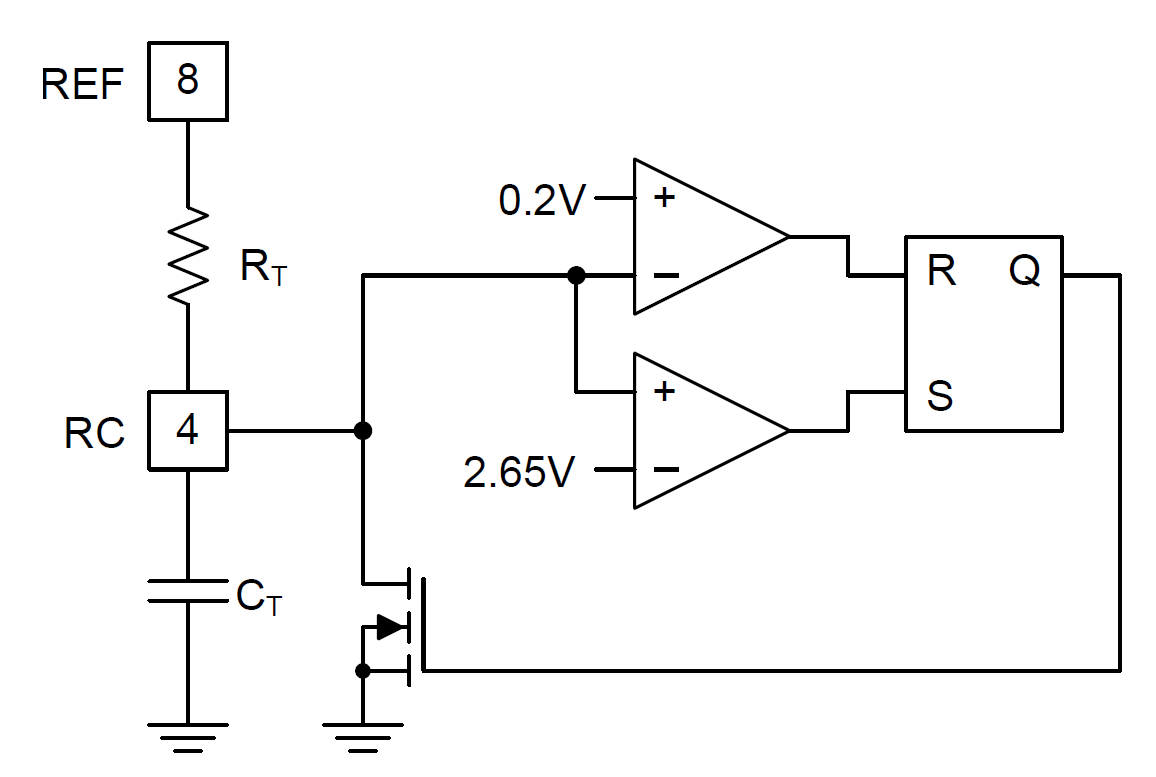
\includegraphics[max width=0.7\linewidth]{/tex/2iteration/billeder/PWM_oscillator_diagram.PNG}
	\caption{Oscillator diagram}
	\label{fig:PWM_oscillator_diagram}
\end{figure}

Figur~\ref{fig:PWM_oscillator_diagram} viser et ækvivalent diagram for oscillator blokken. Komponenterne $R_T$ og $C_T$ er det eksterne RC kredsløb, mens resten er interne komponenter. På diagrammet ses det at operationsforstærkerne er koblet til henholdsvis $0.2V$ og $2.65V$. Dette sætter maksimum og minimum for savtand spændingen. 

Da der skal komme en flanke på output-signalet hver gang savtand spændingen rammer maksimum, skal frekvensen af savtand spændingen være den dobbelte af den ønskede switch-frekvens. Der ønskes en switch-frekvens på $100k\hertz$, derfor sættes oscillator frekvensen til $f_{osc}=200k\hertz$. I databladet er det anbefalet at $R_T$ vælges mellem $10k\ohm$ og $200k\ohm$, mens det anbefales at $C_T$ vælges mellem $100p\farad$ og $1000p\farad$. Formel~\ref{f_osc} er opgivet i databladet og bruges til at estimere RC komponenterne. $C_T$ sættes til $200p\farad$, og $R_T$ beregnes:
\begin{equation} \label{f_osc}
R_{T} = \frac{1.5}{f_{osc} \cdot C_T} = \frac{1.5}{f_{osc} \cdot C_T} = 37.5k\ohm
\end{equation}
Ved et opslag i databladet ses det, at med en $C_T=200p\farad$ kan der maksimalt opnås en duty-cycle på ca. $48.9\percent$. Da converteren maksimalt skal opererer med en duty-cycle på $44.7\percent$, godtages dette.

\subsection{Current sense kredsløb} \label{CS_loop}
Som nævnt i afsnit~\ref{PWM} er der valgt at bruge peak-current regulering. Denne form for regulering består af to reguleringssløjfer - en spændings- og en strømsløjfe. I dette afsnit beskrives dimensioneringen af strøm sløjfen, mens spændingssløjfen beskrives i afsnit~\ref{V_loop}.

Current sense kredsløbet består, som minimum, af en current sense modstand. Denne modstand bruge til at konvertere strømmen i transformatorens primærvikling om til en spænding. Denne konvertering vil gøre, at kurveformen for strømmen og spændingen er ens, dog med en faktor til forskel. PWM-komparatoren i controlleren trigger udgangen, når current sense spændingen er rampet op til $1V$. Derfor skal modstanden dimensioneres således, spændingen over den er lig $1V$ når peak-strømmen i transformatoren er lig $5.53A$. Dette regnes ud fra Ohm's lov:
\begin{equation} \label{R_cs}
R_{cs} = \frac{1V}{5.53A} = 0.181\ohm
\end{equation}

Da den mindste modstandsværdi der er til rådighed er på $1\ohm$, vil der blive brugt $6\cdot 1\ohm$ i parallel. Dette vli give en modstandsværdi på $0.167\ohm$. 



\subsubsection{Filtrering}
På grund af switching-spikes i MOSFET'en, når den går ON, vil der også komme spikes på current sense signalet. Hvis disse spikes når et niveau der er højere end $1V$, vil det trigger komparatoren. Dette vil få controlleren til at generer et PWM-signal, der er meget lavere end det ønskede. Derfor implementeres der et filter, for at filtrere disse spikes væk.

UCC1801 har et indbygget digitalt filter, kaldet Leading Edge Blanking. Dette filter er designet til at filtrere de første $100ns$ af signalet væk, og dermed fjerne spiken. Ideelt set vil dette give et signal, som ses på figur~\ref{fig:ucc1801_leading_edge}.

\begin{figure}[H]
	\center
	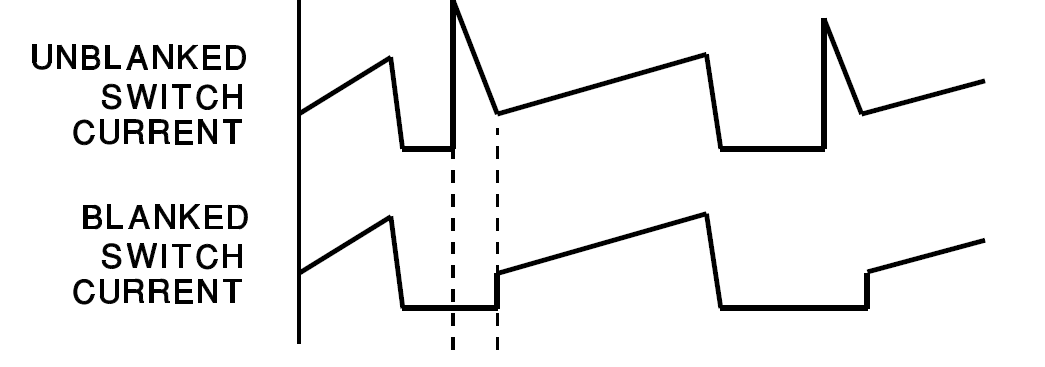
\includegraphics[max width=0.7\linewidth]{/tex/2iteration/billeder/ucc1801_leading_edge.PNG}
	\caption{Current sense signal før og efter Leading Edge Blanking}
	\label{fig:ucc1801_leading_edge}
\end{figure}

Det digitale filter er ikke altid tilstrækkeligt, og derfor designes et eksternt analogt RC-filter, for yderligere filtrering. Det designes til at have en stige tid på $300ns$, for at tilføje en yderligere filtrering på ca. $200ns$. 

\noindent Med en stige tid på $300ns$, kan båndbredden af filteret estimeres:
\begin{equation} \label{filter_BW}
BW \approx \frac{0.34}{t_r} \approx 1.133M\hertz
\end{equation}

\noindent Der vælges en kondensator på $C_f=100pF$. Ud fra kondensatoren og den ønskede båndbredde i filteret, regnes modstanden.
\begin{equation} \label{filter_R}
R_f = \frac{1}{2 \cdot \pi \cdot BW \cdot C_f} = 1.4k\ohm
\end{equation}

Med det designede filter vil stige tiden af current sense signalet, nu blive begrænset af filteret. Derfor vil den første de af signalet nu ligne et første ordens system, der stiger indtil spændingen når det niveau der svarer til strømmen i primærviklingen. Derefter vil signalet stige som en ret linje, ligesom strømmen. Dette ses på figur~\ref{fig:ucc1801_CS_filter}, hvor det øverste signal er før filteret, og det nederste er efter.

\begin{figure}[H]
	\center
	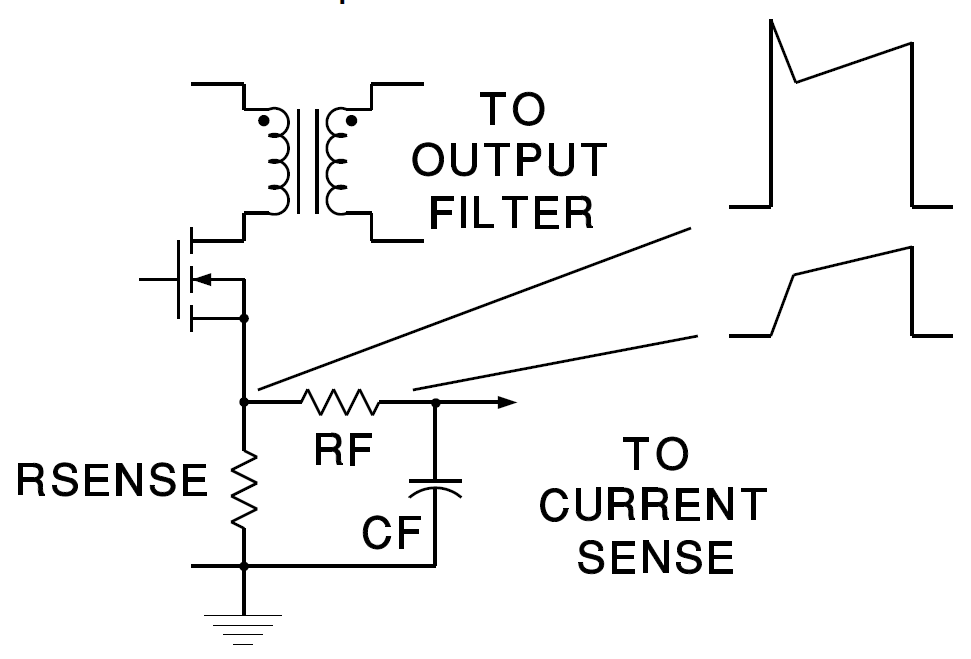
\includegraphics[max width=0.7\linewidth]{/tex/2iteration/billeder/ucc1801_CS_filter.PNG}
	\caption{Current sense signal før og efter eksternt RC-filter}
	\label{fig:ucc1801_CS_filter}
\end{figure}

\subsubsection{Overstrømsbeskyttelse} \label{CS_protection}
En fordel ved, at regulere efter strømmen i transformatoren er, at der opnås en overstrømsbeskyttelse. Når strømmen stiger, vil PWM-controlleren sænke duty-cyclen, og derved også sænke udgangsspændingen. Dette giver en I/V karakteristik der, ideelt set, er næsten firkantet. Dette er skitseret på figur~\ref{fig:I-V_karateristik}. 

\begin{figure}[H]
	\center
	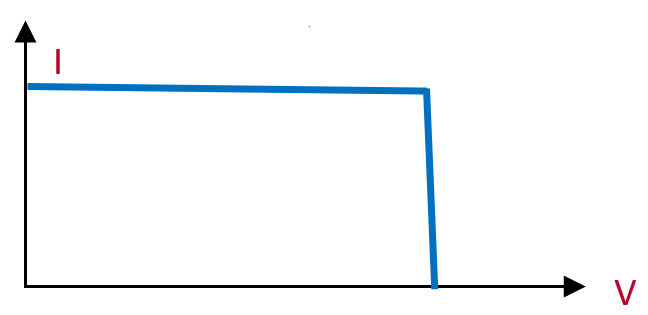
\includegraphics[max width=0.7\linewidth]{/tex/2iteration/billeder/I-V_karakteristik.PNG}
	\caption{I/V karakteristik for converteren}
	\label{fig:I-V_karateristik}
\end{figure}

Denne karakteristik kan dog ikke opnås i realiteten. Filteret der er indsat for at filtrere current sense signalet, vil lave en hale på karakteristikken. Det sker fordi controlleren ikke ser den faktiske strøm, men den filtrerede, når duty-cyclen er lav. 

Da det er nødvendigt at filtrere current sense signalet, men samtidig påvirker converterens I/V karakteristik, optimeres filteret ofte således, det kun akkurat filtrer nok. Denne optimering vil ske i 3. iteration. 

\subsection{Spændingsregulering} \label{V_loop}
I dette afsnit beskrives spændingssløjfen. Den består hovedsageligt af to dele: en spændingsdeler og en fejlforstærker. Spændingsdeleren deler udgangsspændingen ned, så den ønskede udgangsspænding er lig en intern reference i IC'en. Fejlforstærkeren står for selve reguleringen. Den inverterende indgang og udgangen på fejlforstærkeren er ført ud, således det er muligt at indsætte et kompenseringsnetværk.

\subsubsection{Spændingsdeler}
Den ikke inverterende indgang på den indbyggede fejlforstærker i UCC1801, er forbundet til den halve reference spænding, dvs. $2.5V$. Derfor skal der designes en spændingsdeler, der deler den ønskede udgangsspænding på $21V$ ned til $2.5V$. Figur~\ref{fig:Voltagedivider_ideal} viser kredsløbet for spændingsdeleren. 

\begin{figure}[H]
	\center
	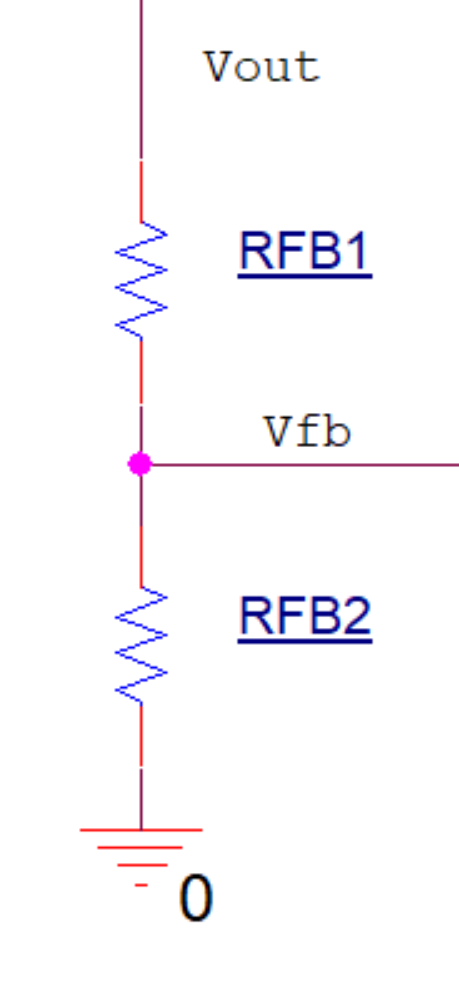
\includegraphics[max width=0.7\linewidth]{/tex/2iteration/billeder/Voltagedivider_ideal.PNG}
	\caption{Spændingsdeler diagram}
	\label{fig:Voltagedivider_ideal}
\end{figure}

Spændingsdeleren designes således der løber en strøm på $1mA$ i den. Derved påvirker den ikke udgangsstrømmen. Derudover dimensioneres de to modstande, således der er et spændingsfald på $2.5V$ over $R_{FB2}$, og $21V-2.5V$ over $R_{FB1}$. $R_{FB1}$ er beregnet med ligning~\ref{RFB1}.

\begin{equation} \label{RFB1}
R_{FB1} = \frac{V_{out}-V_{FB}}{I_{FB1}} = \frac{21V-2.5V}{1mA} = 18.5k\ohm
\end{equation}

\noindent $R_{FB2}$ er beregnet ud fra spændingsdeler formlen, ligning~\ref{RFB2}. Her løses $R_{FB2}$, og fås til $R_{FB2}=2.527k \ohm$.  
\begin{equation} \label{RFB2}
V_{FB} = \frac{R_{FB2}}{R_{FB1} + R_{RB2}} \cdot V_{out}
\end{equation}

For at opnå en præcis spændingsdeler vælges der at bruge to modstande i parallel. Den ene modstand vælges til $R_{FB21}=2.55k\ohm$. Mens den anden regnes ud fra den ønskede samlede modstandsværdi. Dette gøres ved ligning~\ref{RFB22}, som løses med hensyn til $R_{FB22}$. Dette giver $R_{FB22}=280.5k\ohm$, som afrundes til $280k\ohm$.
\begin{equation} \label{RFB22}
R_{FB2} = ((R_{FB21})^{-1} + (R_{FB22})^{-1})^{-1}
\end{equation}

\subsubsection{Fejlforstærker}
Som en del af reguleringen opstilles der først en overføringsfunktion for power-modulet. Denne overføringsfunktion er opgivet i databladet for UCC1801, og er skrevet ved ligning~\ref{H_Power}.
\begin{equation} \label{H_Power}
G_{pwr}(s) = G_0 \cdot \frac{(1+\frac{s}{2\pi \cdot f_{ESRz}}) \cdot (1-\frac{s}{2\pi \cdot f_{RHPz}})}{1+\frac{s}{2\pi \cdot f_{p1}}} \cdot \frac{1}{1 + \frac{s}{2\pi \cdot f_{p2}} + \frac{s^2}{(2\pi \cdot f_{p2})^2}}
\end{equation}

Overføringsfunktionen består af flere dele: en DC-forstærkning, to poler og to nulpunkter. DC-forstærkningen, $G_0$, er skrevet ved ligning~\ref{DC_gain}. Den er især bestemt af belastningen, current sense kredsløbet, transformatoren og switch-frekvensen. Den regnes til en forstærkning på $10.74$ gange, eller $20.6\decibel$.
\begin{equation} \label{DC_gain}
G_0 = \frac{R_{out} \cdot N}{R_{CS} \cdot A_{CS}} \cdot \frac{1}{\frac{(1-D)^2}{\tau_L} + (2 \cdot M) + 1} = 10.7GG \Rightarrow 20.6\decibel
\end{equation}
\noindent Hvor:
\newline \noindent $N$ er omsætningsforholdet i transformatoren.
\newline \noindent $A_{CS}$ er den interne forstærkning i current sense kredsløbet, og aflæses i databladet til $1.65$.
\newline \noindent $D$ er den maksimale duty-cycle, som er $0.447$.
\newline \noindent $\tau_L$ er converterens tidskonstant. Den regnes ud fra ligning~\ref{tau_L}.
\begin{equation} \label{tau_L}
\tau_L = \frac{2 \cdot L_P \cdot f_s}{R_{out} \cdot N^2}
\end{equation}
\newline \noindent $M$ er spændingsomsætningen fra indgang til udgang. Den regnes ud fra ligning~\ref{M}.
\begin{equation} \label{M}
M = \frac{V_{out} \cdot N}{V_{in}}
\end{equation}

En flyback converter, som opererer i CCM, har to primære nulpunkter der kan påvirke stabiliteten i systemet. Det er også de to nulpunkter der er inkluderet i overføringsfunktionen. Den ene, $f_{ESRz}$, er bestemt af produktet mellem udgangskapaciteten og den indre seriemodstand i udgangskondensatoren. Placeringen af denne er regnet ved ligning~\ref{ESR_zero}.
\begin{equation} \label{ESR_zero}
f_{ESRz} = \frac{1}{2 \cdot \pi \cdot R_{ESR} \cdot C_{out}} = 189.5k\hertz
\end{equation}

Det andet nulpunkt er højre-halvplans-nulpunktet. Det er ofte dette nulpunkt der er det dominerende af de to, og derfor den der skal tages højde for i reguleringen. Placeringen af dette er regnet ved ligning~\ref{RHP_zero}. Placeringen af dette nulpunkt, er afhængigt af størrelsen på belastningen, samt inputspændingen. Placeringen stiger ved højere inputspændinger, og mindre belastninger. 
\begin{equation} \label{RHP_zero}
f_{RHPz} = \frac{R_{out} \cdot (1-D)^2 \cdot N^2}{2 \cdot \pi \cdot L_P \cdot D} = 15.8k\hertz
\end{equation}

\noindent Ud fra ligning~\ref{ESR_zero} og \ref{RHP_zero}, ses det, at det er højre-halvplans nulpunktet der er det dominerende nulpunkt i converteren. Når båndbredden skal vælges, er det derfor vigtigt, at den ligger tilpas meget lavere end det dominerende nulpunkt.

Converteren har også to relevante poler. Den dominerende pol bestemmes af load'en og udgangskondensatoren. Den anden pol er placeret ved den halve switching-frekvens. De to poler er beregnet ved ligning~\ref{pol1} og \ref{pol2}.
\begin{equation} \label{pol1}
f_{p1} = \frac{\frac{(1-D)^3}{\tau_L} + 1 + D}{2\cdot \pi \cdot R_{out} \cdot C_{out}} = 132.8\hertz
\end{equation}

\begin{equation} \label{pol2}
f_{p2} = \frac{f_s}{2} = 50k\hertz
\end{equation}

\noindent Bode plottet for power-modulet plottes i MATLAB på figur~\ref{fig:MATLAB_power_module}. Her aflæses DC-forstærkningen til $20.6\decibel$. Derudover aflæses der en pol ved ca. $130\hertz$ og ved ca. $50k\hertz$. Dette stemmer overens med de beregnede værdier.

Konsekvensen af højre-halvplans nulpunktet ses også tydeligt på figur~\ref{fig:MATLAB_power_module}. Når frekvensen nærmer sig nulpunktet bliver forstærkningen øget med $20 \decibel$/decade, som ved et venstre-halvplans nulpunkt. Tilgengæld vil fasen blive trukket ned med $90^\circ$, i stedet for op. Da polen fra switch-frekvensen ligger ca. samme sted, og også trækker fasen ned med $90^\circ$, kommer der et stort fasedrej i dette frekvensområde. Det kan gøre systemet ustabilt hvis gain-marginen ikke er tilstrækkelig stor. 

\begin{figure}[H]
	\center
	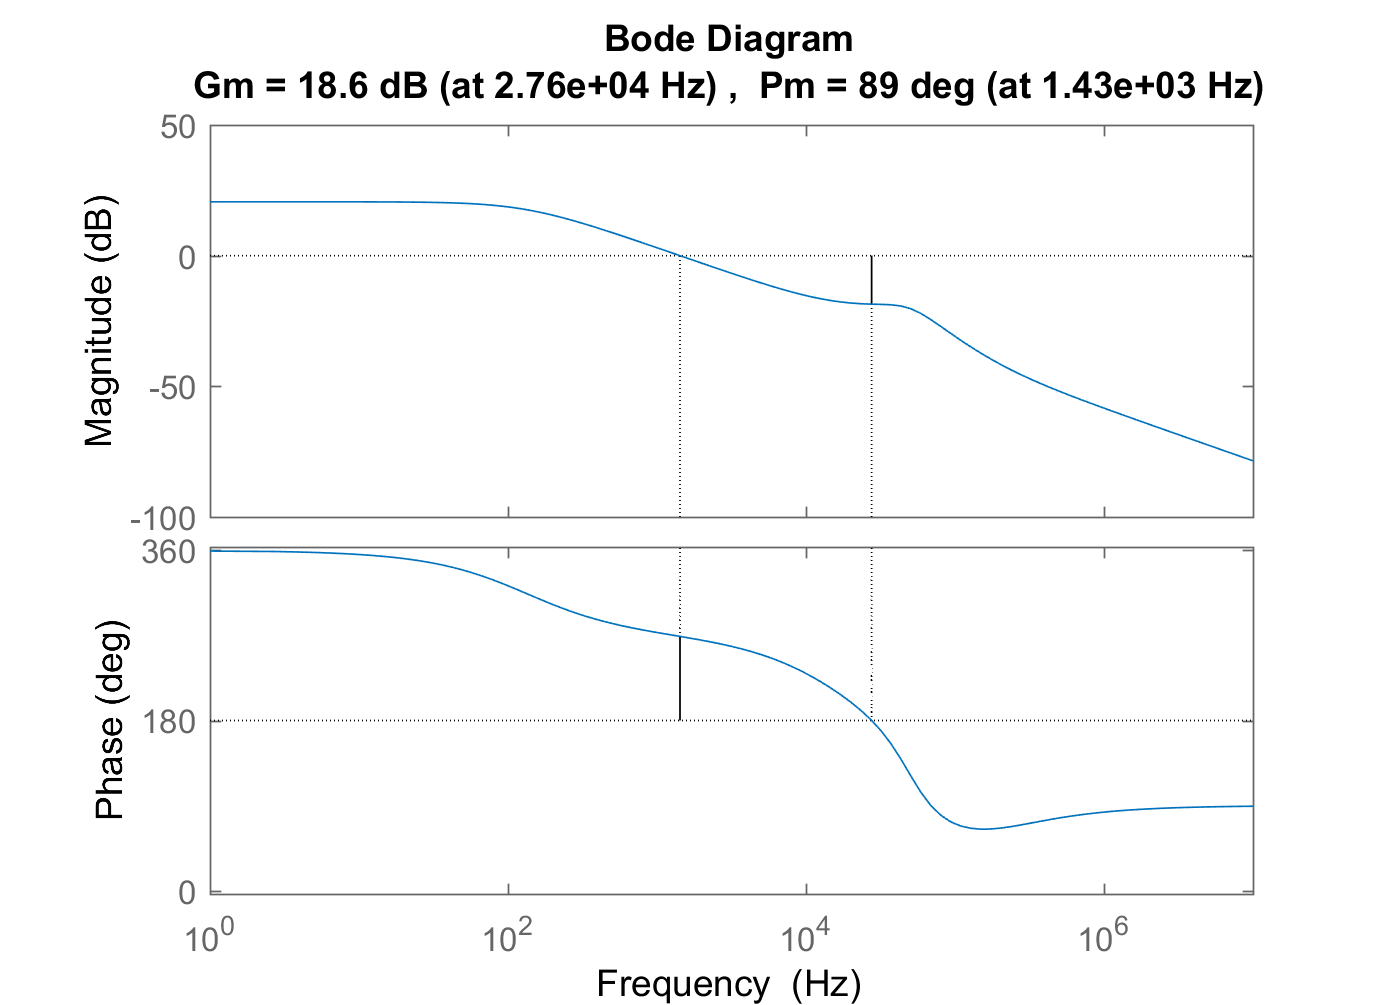
\includegraphics[max width=0.7\linewidth]{/tex/2iteration/billeder/MATLAB_power_module.PNG}
	\caption{Bode plot for power-modulet}
	\label{fig:MATLAB_power_module}
\end{figure}

I denne iteration designes der et kompensationsnetværk der vil sikre et stabilt system, med en lav båndbredde. Dette vil blive optimeret i en senere iteration. 
Da der ønskes en lavere båndbredde, end det converteren har i forvejen, indsættes et RC-led i serie som kompensationsnetværk. Ved at bruge et RC-led, vil kondensatoren bestemme forstærkningen ved lave frekvenser, fordi impedansen her er stor. Mens modstanden vil bestemme forstærkningen ved høje frekvenser, fordi kondensatoren vil blive set som en kortslutning. 

Den endelige båndbredde af systemet ønskes på ca. $800\hertz$. Det vil sikre, at systemet ikke bliver ustabilt. For at opnå den ønskede båndbredde aflæses det ud fra bode plottet på figur~\ref{fig:MATLAB_power_module}, at forstærkningen skal mindskes med ca. $5.4\decibel$, eller ca. $0.535GG$, ved frekvenser over $800\hertz$. Den samlede forstærkning af reguleringssløjfen, bestemmes af produktet mellem forstærkningen i spændingsdeleren og forstærkningen i fejlforstærkeren. Forstærkningen i spændingsdeleren regnes ved ligning~\ref{voltagedivider_gain}.
\begin{equation} \label{voltagedivider_gain}
g_{FB} = \frac{R_{FB2}}{R_{FB1}+R_{FB2}} = 0.12
\end{equation}

\noindent Nu kan feedback modstanden i fejlforstærkeren regnes ved ligning~\ref{error_opamp_gain}. 
\begin{equation} \label{error_opamp_gain}
g_{tot} = \frac{R_{comp}}{R_{par}} \cdot g_{FB}
\end{equation}

\noindent Hvor:
\newline \noindent $g_{tot}$ er det ønskede gain i fejlforstærkeren, som er $g_{tot}=0.535GG$.
\newline \noindent $R_{comp}$ er feedback modstanden i fejlforstærkeren, som ønskes dimensioneret.
\newline \noindent $R_{par}$ er parallelmodstanden mellem $R_{FB1}$ og $R_{FB2}$. Den regnes til $R_{par}=2.244k\ohm$.

\noindent De kendte værdier indsættes og ligningen løses for $R_{comp}$. Den fås til $R_{comp}\approx 10k\ohm$.


\noindent For at sikre en den lave båndbredde, sættes knækfrekvensen på integratoren til $f_0=300\hertz$. Dermed sikres det, at fejlforstærkeren dæmper signalet ved den ønskede båndbredde på $800\hertz$. Nu den tilhørende kapacitet regnes, ud fra $R_{comp}$ og $f_0$.
\begin{equation} \label{c_comp}
c_{comp} = \frac{1}{2\cdot \pi \cdot R_{comp} \cdot f_0} \approx 50nF
\end{equation}

\noindent Med afrundede komponentværdier, regnes den nye knækfrekvens for fejlforstærkeren.
\begin{equation} \label{f_0}
f_0 = \frac{1}{2\cdot \pi \cdot R_{comp}} \cdot c_{comp} = 318.3\hertz
\end{equation}

\noindent Overføringsfunktionen for fejlforstærkeren kan nu opskrives ved ligning~\ref{H_err}.
\begin{equation} \label{H_err}
G_{err}(s) = (\frac{318.3\hertz \cdot 2\cdot\pi}{s} + 1) \cdot 0.535
\end{equation}

\noindent Den plottes i MATLAB, som et bode plot på figur~\ref{fig:MATLAB_error_op_amp_2}. Her ses det, at den ønskede funktion af integratoren er opnået. På grund af kondensatoren, har den et stort gain ved lave frekvenser. Mens forstærkningen ligger konstant ved ca. $-5.4\decibel$, efter den ønskede knækfrekvens på ca. $318\hertz$.

\begin{figure}[H]
	\center
	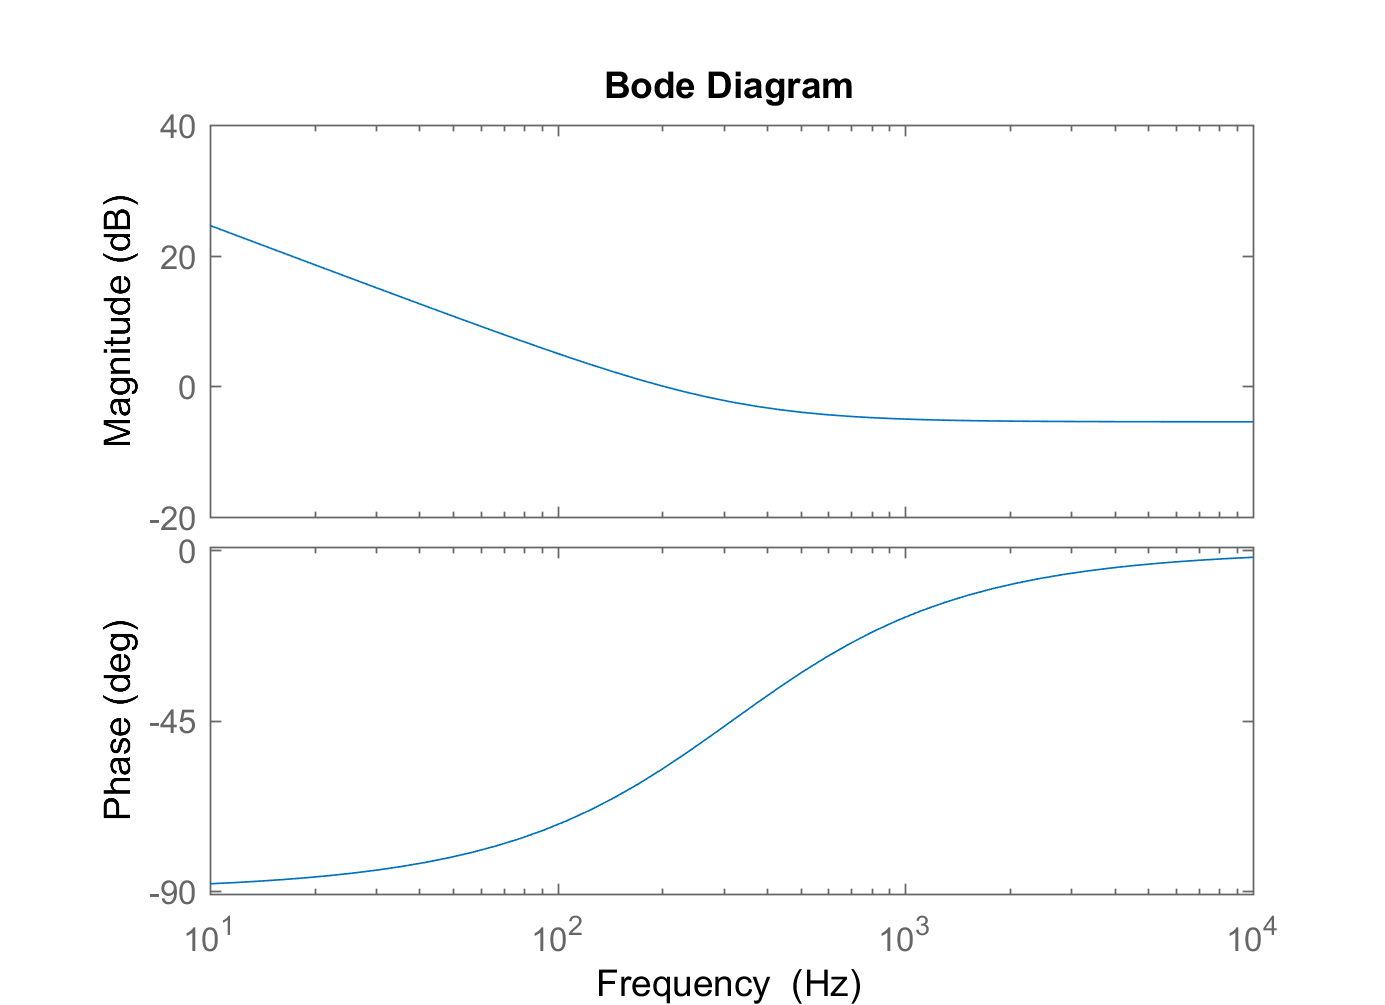
\includegraphics[max width=0.7\linewidth]{/tex/2iteration/billeder/MATLAB_error_op_amp.PNG}
	\caption{Bode plot for fejlforstærker}
	\label{fig:MATLAB_error_op_amp_2}
\end{figure}

De to overføringsfunktioner ganges sammen for, at bestemme den samlede overføringsfunktion for converteren. Figur~\ref{fig:MATLAB_total_2} viser et åben sløjfe bode plot af det. Det aflæses at converteren vil have en båndbredde på $810\hertz$. Derudover aflæses fase-margin til $74.3^\circ$, og gain-margin til $24\decibel$.

\begin{figure}[H]
	\center
	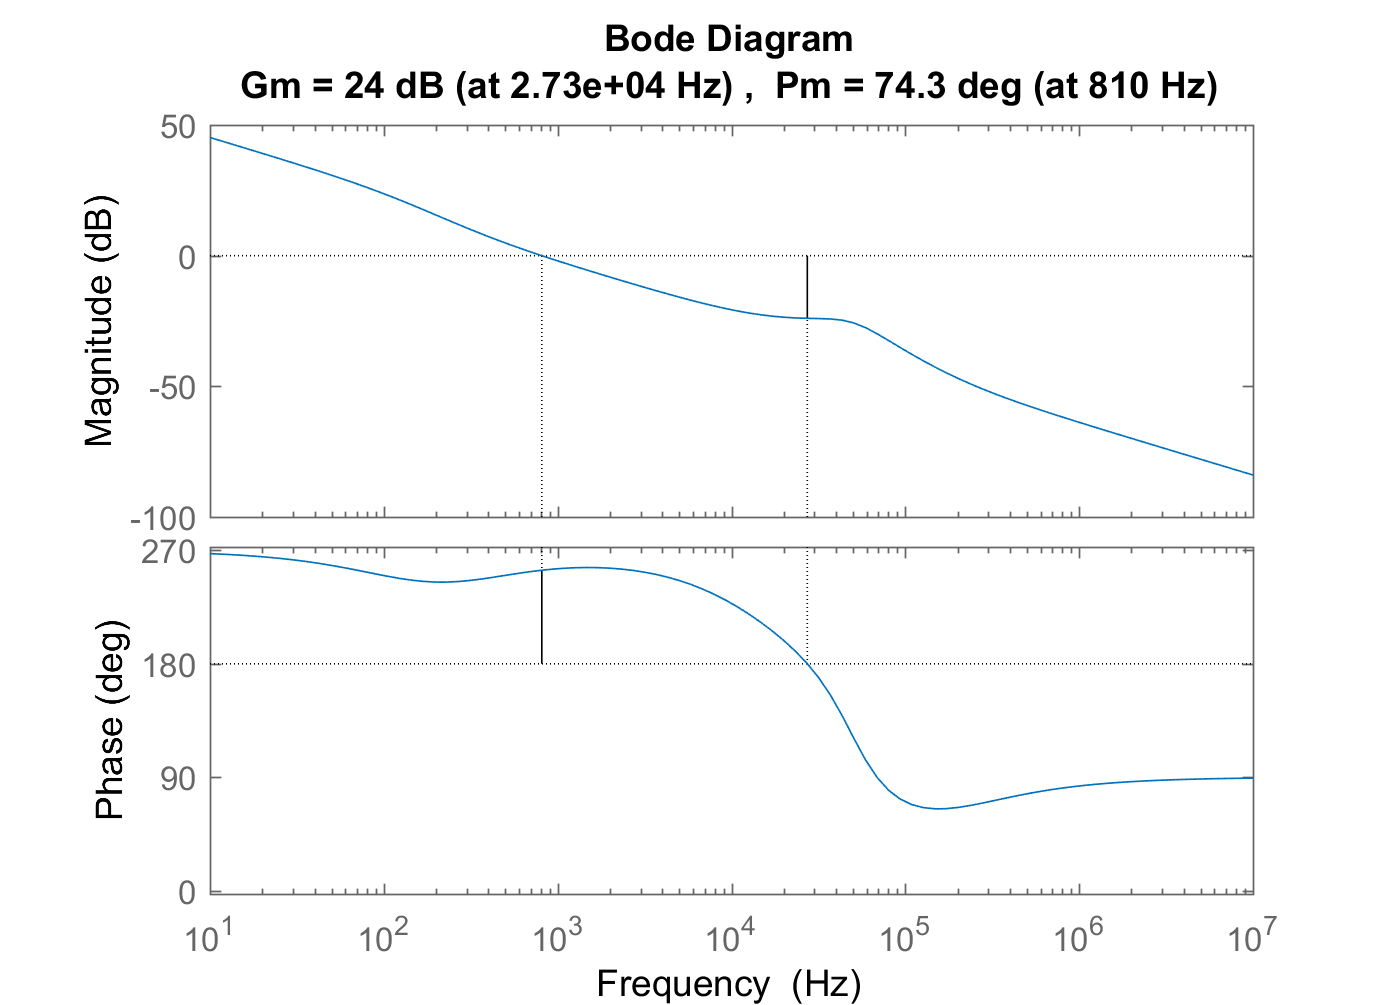
\includegraphics[max width=0.7\linewidth]{/tex/2iteration/billeder/MATLAB_total.PNG}
	\caption{Bode plot for converteren}
	\label{fig:MATLAB_total_2}
\end{figure} 





\subsection{Regulering}
Efter 2. iteration blev besluttet at optimere converterens båndbredde, da der var en stor margin til kravene for både gain- og fasemargin. Med en større båndbredde, ville der samtidig opnås en hurtigere responstid i systemet. 

For design af det nye kompensationsnetværk, blev der taget udgangspunkt i bode plottet for power-modulet. Ud fra kravene for converterens stabilitet, kunne det ses, at der kunne tilføres en forstærkning på $8.6\decibel$, og stadig overholde kravene for gain- og fasemargin. Samtidig blev knækfrekvensen for fejlforstærkeren flyttet til $132.8\hertz$, da den dominerende pol for converteren lå her. 

For at opnå den ønskede forstærkning på $8.6\decibel$, eller $2.66gg$, regnes modstanden i kompensationsnetværket til $R_{comp} = 49.8k\ohm$. For at opnå den valgte knækfrekvens regnes kondensatoren til $24.2nF$. 

For en mere detaljeret gennemgang af overføringsfunktionernes indhold, og deres bode plots, henvises til dokumentationens afsnit 6.5 og 6.8.5.


\input{tex/Implementering/2iteration/MOSdiodekon}

\section{Tab}
Dette afsnit omhandler de overvejelser, der er gjort omkring tab i 2. iteration. Her omtales hvilke bidrag, der er taget højde for, til udberegninger af tab for de enkelte komponenter. Udregningerne og yderligere forklaring af disse, kan findes dokumentationen afsnit 5.7.

\subsubsection{Transformator}
Tabet i transformatoren er set som to dele. Et kernetab og et kobbertab. Kernetabet afhænger af  kernematerialet, selvinduktionen og strømmen i viklingerne. Disse bruges til at udregne fluxen i kernen. Med denne værdi og databladskurven for det specifikke tab som funktion af maks flux massefylden, er kernetabet blevet estimeret. 

Kobbertabet kommer af modstanden, der er i kobbertrådene, som er viklet om kernen. Dette indebærer både bidrag fra en DC modstand og en AC modstand. DC modstanden er udregnet ud fra længden og tykkelsen af kobbertrådene. AC modstanden opstår på grund af magnetfeltet kobbertrådene ligger i. AC modstandens del af kobbertabet er der i dette projket ikke valgt at tage højde for.

Det samlede tab for transformatoren er testet, ved at måle temperaturen på kernen efter converteren har været i gang over længere tid. Med en datablads værdi af den termiske modstand for en RM8 kerne er tabet herefter udregnet.   

\subsubsection{MOSFET}
MOSFET'ens tab kan ligeledes deles op i to centrale bidrag; 

conduction tab og switchtab. Conduction tabet kommer af RMS strømmen der løber i MOSFET'ens ON modstand. 

Switchtabet kommer som konsekvens af effekttrekanterne, der opstår, imellem MOSFET'ens ON og OFF perioder. Effekttrekanterne er i dette projekt estimeret ved at udregne dem som arealet af to lige store trekanter. Højden på trekanten er peakaverage strømmen ganget med den maksimale spænding der vil ligge over MOSFET'en. Længden af trekanten fås af den samlede switch-tid i forhold til den samlede switch periode. 

Det samlede tab i MOSFET'en er testet ved at måle temperaturen på kølepladen efter converteren har været i gang over længere tid. Denne temperaturstigning ganget med køle-koefficienten for kølepladen giver tabet. 

\subsubsection{Diode}
Tabet i dioden er udregnet ved, at kigge på spændingsfaldet over dioden ganget udgangsstrømmen. Som nævnt benyttes en schottky diode, og der har derfor ikke været behov for betragtninger af switch-tabet i dioden. 

Tabet for dioden er fundet ved at måle temperaturen af kølepladen ligesom ved MOSFET'en ovenfor.   

\subsubsection{Kondensator}
Med en kendt ESR modstand for kondensatoren, har det været muligt at beregne tabet i denne. Da modstanden er så lille, er tabet dog uden betydning for det samlede tab.

\subsubsection{Current-sence tab}
Tabet i current-sence modstanden er udregnet ved modstandsværdien ganget med RMS strømmen i anden. Strømmen i igennem modstanden er den samme som løber i den primære vikling. 

\subsubsection{Samlet tab}
De ovenstående tab er alle analyseret og simuleret. Derudover er der lavet test af de tab, hvor det var muligt. Resultatet af dette ses i resultatafsnittet \fxnote{indsæt resultatafsnit for tab}.
Det samlede tab for converteren i 2. iteration er i analyse og simulering fundet ved at lægge de fundne tab sammen. I testen er der set på den effekt der sendes ind i converteren og trukket udgangseffekten fra denne.



\section{Integrationstest} \label{Integrationstest}
Der er lavet tre forskellige test af det samlede system, til at teste de essentielle funktioner af converteren. Det drejer sig om constant-load, gain-fase måling og load-step. For nærmere beskrivelse af hver enkelt test, henvises til dokumentationen afsnit 5.9.

På figur~\ref{fig:sche2iteration} ses et schematic for det samlede implementerede kredsløb for 2. iteration.
\begin{figure}[H]
	\center
	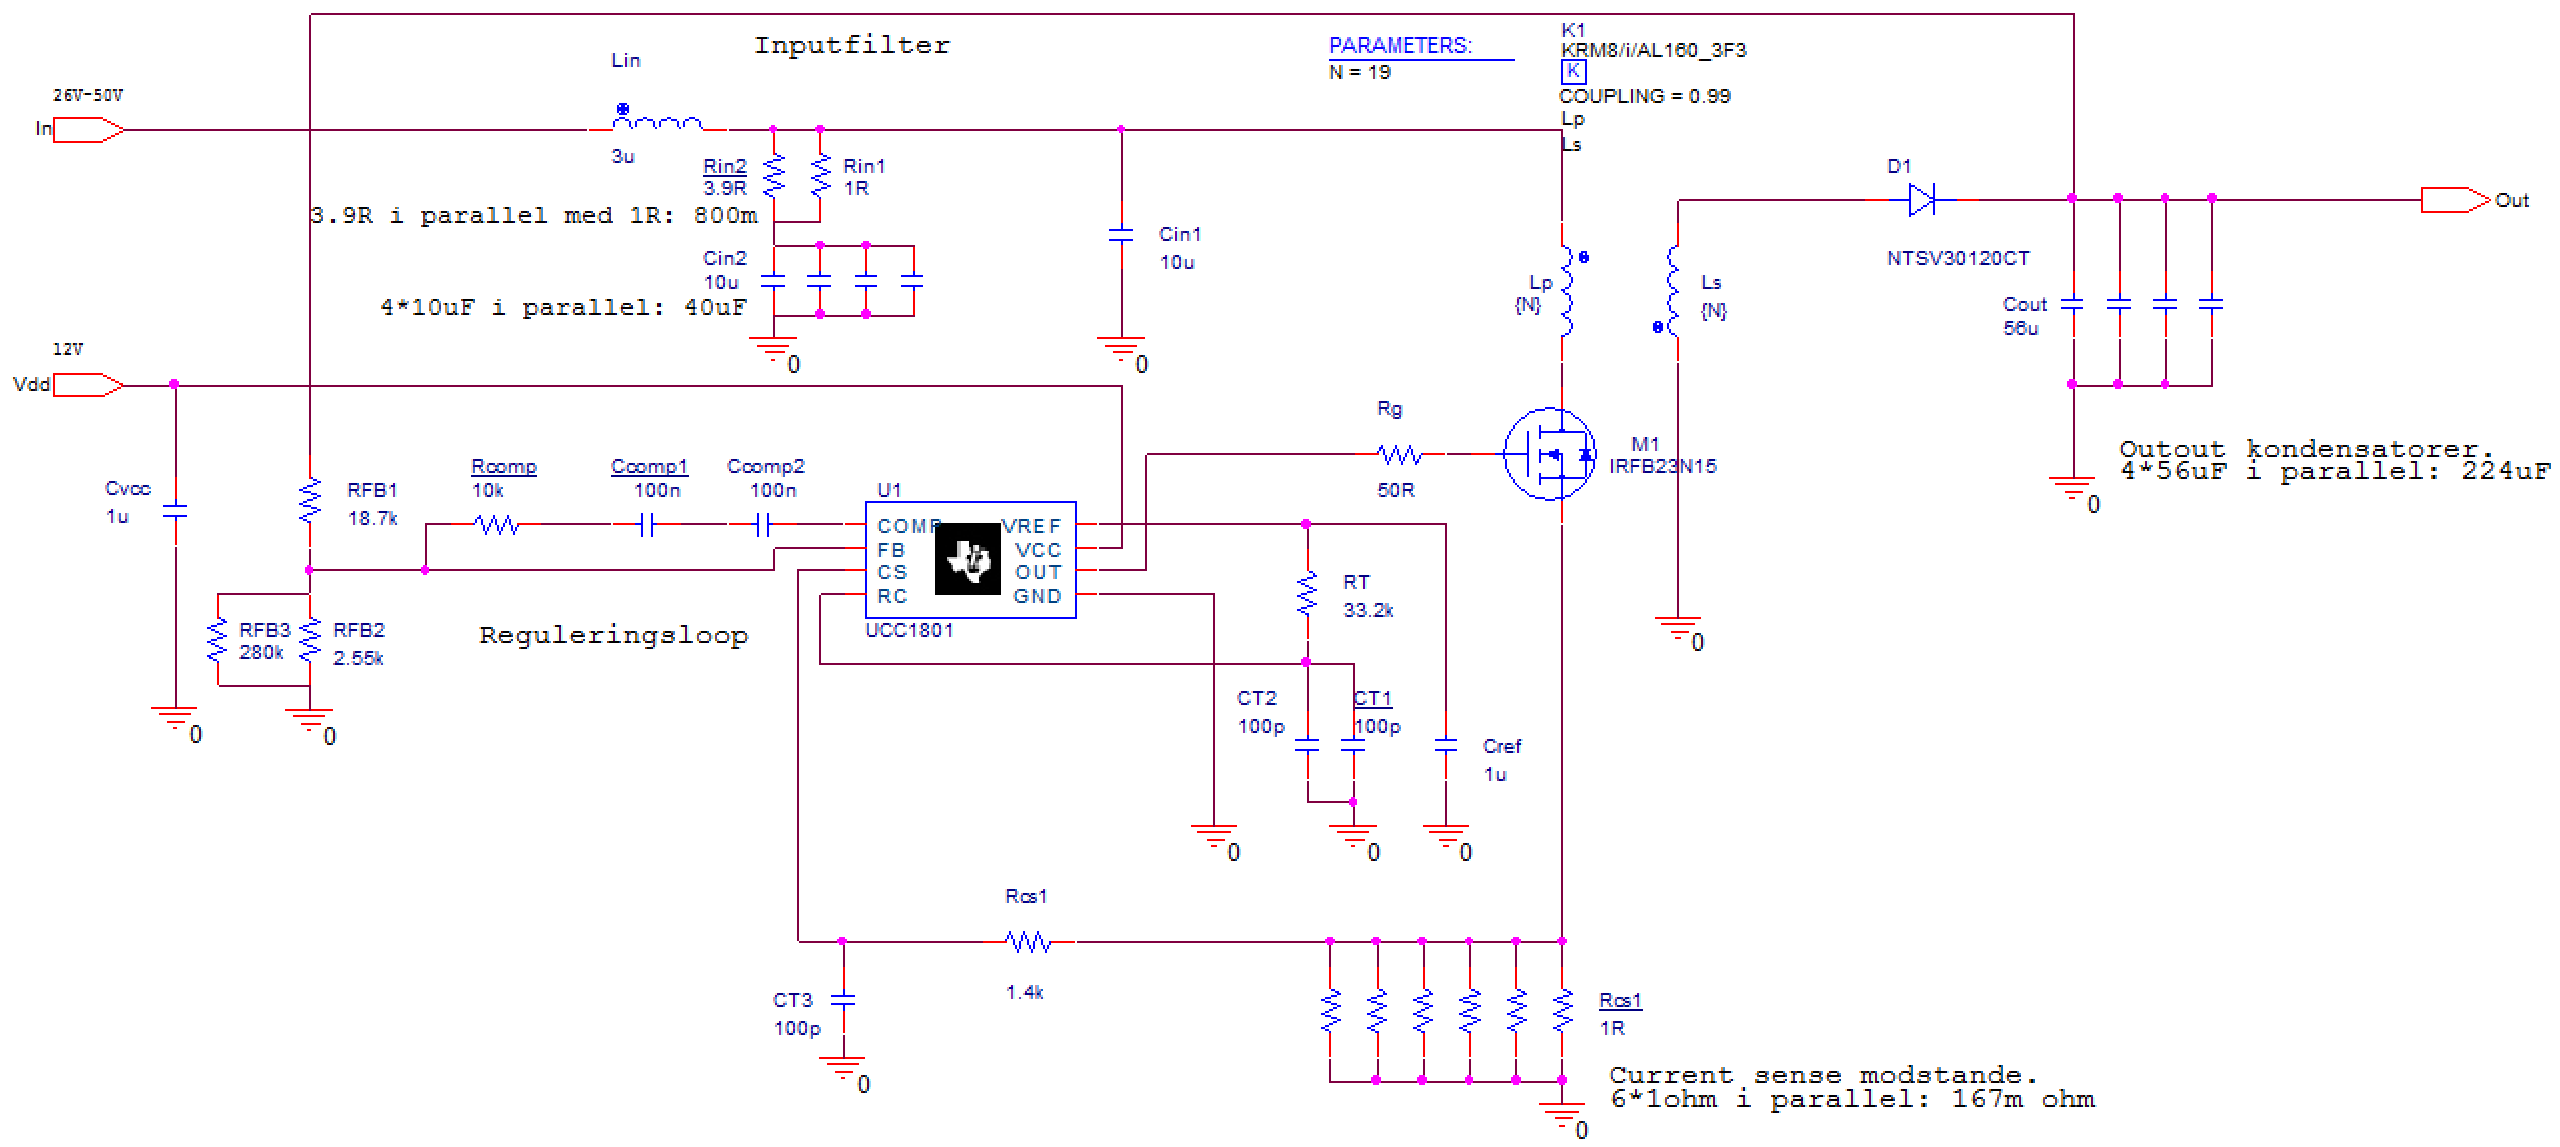
\includegraphics[max width=1.1\linewidth]{../dokumentation/tex/2iteration/billeder/Schemaricoverview_2iteration.PNG}
	\caption{Schematic overblik for 2. iteration}
	\label{fig:sche2iteration}
\end{figure}

\subsection{Constant-load}
Ved testen constant-load måles interessante steder i systemet, hvor en konstant belastning bruges. Her er en belastning på $8.4\ohm$ benyttet, med en indgangsspænding på 26V, med mindre andet er opgivet.

Ved testen er spændingen over outputtet, MOSFET'en og dioden målt. Desuden er der lavet målinger på de centrale dele af PWM-controlleren. Det indebærer målinger af switch-frekvensen, switch-tiden og stigetiden på filtret til current-sense signalet.  
Ved testen er converterens tab samtidig fundet. Tabet for transformator, MOSFET og diode er fået ved at måle temperaturen af den enkelte komponent, efter converteren har været kørende i længere tid. Temperaturstigningen er sammen med kølepladernes kølekoefficienter, og transformatorens termiske modstand, brugt til beregning af tab. Det samlede tab for converteren i 2. iteration, er i analyse og simulering fundet ved, at lægge de fundne tab sammen. I testen er der set på den effekt, der sendes ind i converteren og trukket udgangseffekten fra denne.

\subsection{Gain-fase måling}
Til gain-fase måling af converteren er Network Analyzeren HP4194A\cite{hp4194} benyttet. Her laves en måling af overføringsfunktionen for power-modul, fejlforstærker og for det samlede system. Det er gjort, ved at indføre et fejlsignal i tilbagekoblingen, og måle hvordan udgangen ændrer sig. Fejlsignalet blev indført med en amplitude på $30mV$. Dette er der lavet et frekvens-sweep på fra, $10\Hz$ til $100kHz$. Målingerne fra Network Analyzeren overføres til et Excel ark, hvor et bode plot er udarbejdet ud fra testmålingerne. 

\subsection{Load-step}
For at lave load-step testen, er der som udgangsbelastning brugt to $20\ohm$ modstande i parallel. Den ene koblet til en switch, så den kan kobles til eller fra. Det gør, at når switchen er OFF, består belastningen af en $20\ohm$ modstand. Når switchen er ON, består den i stedet af en $10\ohm$ modstand. Switchen var indstillet til at sende en puls på 10ms.

\noindent Ved denne test er det spændingsændringen på outputtet der er målt.


\clearpage

\section{Tredje iteration}
Målet for 3. iteration var, at optimere på converterens effekttab, båndbredde og udgangsens switching-spikes. Desuden blev det prioriteret at fjerne ringninger på drain- og anode spændinger, ifm. switching. Disse optimeringer er foretaget på baggrund af de diskuterede resultater fra 2. iteration i afsnit~\ref{diskussion}.
Kravet for at gå videre til 4. iteration var opnåelse af et tilfredsstillende resultat ifm. disse optimeringer.


\subsection{Switch-tid}
Efter 2. iteration blev det besluttet, at optimere effekttabet i converteren. Ud fra tabsmålingerne kunne det ses, at switch-tabet i MOSFET'en, var den dominerende faktor i det samlede effekttab. Det blev valgt, at mindske switch-tiden til lidt under en tredjedel af udgangspunktet fra 2. iteration. Det ville mindske switch-tabet betydeligt. Samtidig vil peak-spændingerne over MOSFET'en stadig overholde dens specifikationer. 

Modstanden, der skulle sikre den hurtigere switch-tid, blev designet efter samme formel som i 2.iteration. Den blev regnet til $13.7\ohm$, hvilket gav en switch-tid på ca. $37.2ns$. 

En nærmere beskrivelse af konsekvenser og designmetode, er beskrevet i dokumentationen, afsnit 6.1.


\subsection{Current-sense filter}
Efter 2. iteration blev det valgt, at optimere stigetiden i current-sense filteret. Det blev gjort for, at fjerne fejlmålinger af strømmen i primærviklingen, og dermed forbedre converterens I/V-karakteristik. 

Ved aflæsning af bredden på spikes på current-sense signalet, blev det valgt, at designe filteret til en stigetid på $100ns$. Ved at fastholde kondensatoren i filteret på $100pF$, blev den nye modstand regent til $464\ohm$. 

En nærmere begrundelse for designvalg og -metode er beskrevet i dokumentationens afsnit 6.2.


\subsection{Snubber-kredsløb}
Der blev designet to snubber-kredsløb for, at fjerne ringninger på spændingen over både MOSFET og diode. De blev anslået som en konsekvens af, at spredningsselvinduktionen fremstår som en serieforbindelse med kapaciteterne over henholdsvis MOSFET'en, dioden og den kapacitive kobling mellem transformatorens viklinger.  

Det blev valgt, at implementere RC-snubbere til både primær- og sekundærsiden. De består af en modstand i serie med en kondensator, som skal placeres over henholdsvis MOSFET og diode. 

Med kendskab til ringningernes frekvens på primærsiden og transformatorens spredningsselvinduktion, blev den resulterende kapacitet regnet til $266.6pF$. Kondensatoren i snubber-kredsløbet blev valgt til en faktor 2 større, end den resulterende kapacitet, for optimal funktionalitet\cite{snubber_design}. Modstanden blev designet således, at dens impedansen var lig impedansen af spredningsselvinduktionen ved ringningsfrekvensen. Hermed blev snubber-kredsløbet designet til $C_{snubM} = 600pF$ og $R_{snubM} = 23.7\ohm$. 

Figur~\ref{fig:snubber_diagram} viser implementeringen af de to snubber-kredsløb. Her vises de specifikke komponentværdier og placeringen af de to kredsløbene.

\begin{figure}[H]
	\centering
	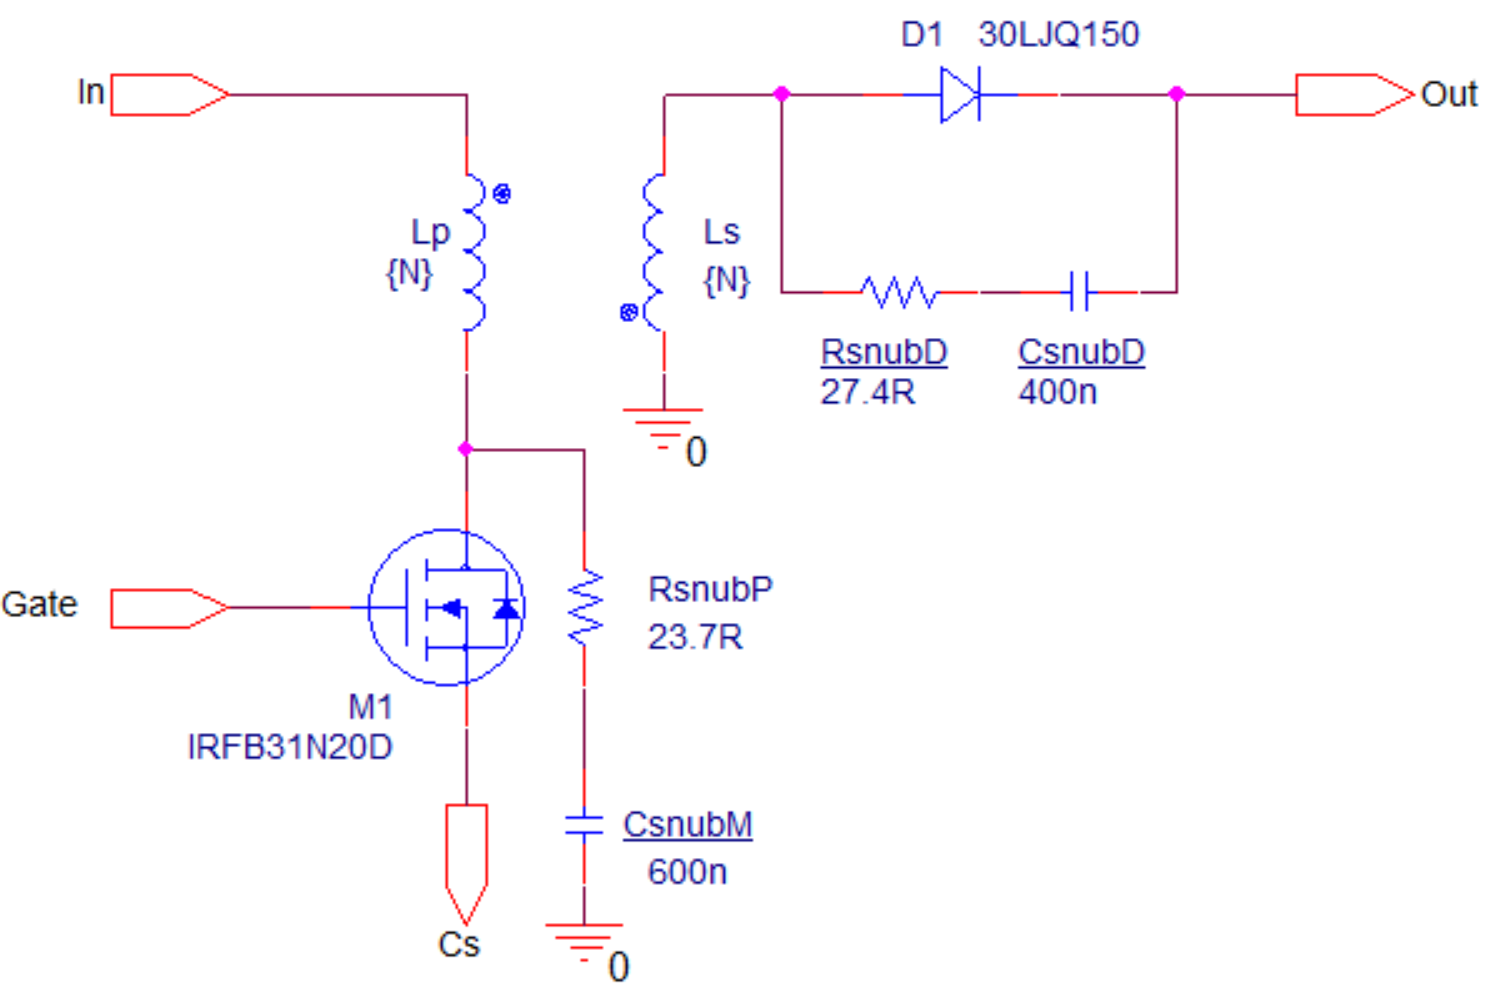
\includegraphics[width=0.4\linewidth]{/tex/Implementering/3iteration/Billeder/Snubber_diagram.png}
	\caption{P-spice diagram for snubber-kredsløb}
	\label{fig:snubber_diagram}
\end{figure}

\noindent Designmetoden for snubber-kredsløbet på sekundærsiden er den samme. Der findes en detaljeret gennemgang af designproceduren og en argumentation for valg af snubber-type i dokumentationen, afsnit 6.3.



\subsection{Udgangsfilter}
I 2. iteration blev det observeret store switching-spikes på udgangssignalet. Derfor blev det besluttet, at tilførere filtrering af disse spikes i 3. iteration. Den nødvendige kapacitet for udgangskondensatoren, blev realiseret ved fire kondensatorer i parallel. Kondensatorerne blev forbundet med ledninger på ca. $30mm$, ses på figur~\ref{fig:udgangsfilter}. Med en tommelfinger regel der siger man har selvinduktion på $1nH/mm$\cite{rule_of_thumb}, vil ledningerne og kondensatorerne derfor skabe fire LC-filtre i serie. Ved at placere udgangen efter disse filtre blev der derfor opnået en filtrering af spikes'ne uden yderligere tilføjelse af komponenter. 

\begin{figure}[H]
	\centering
	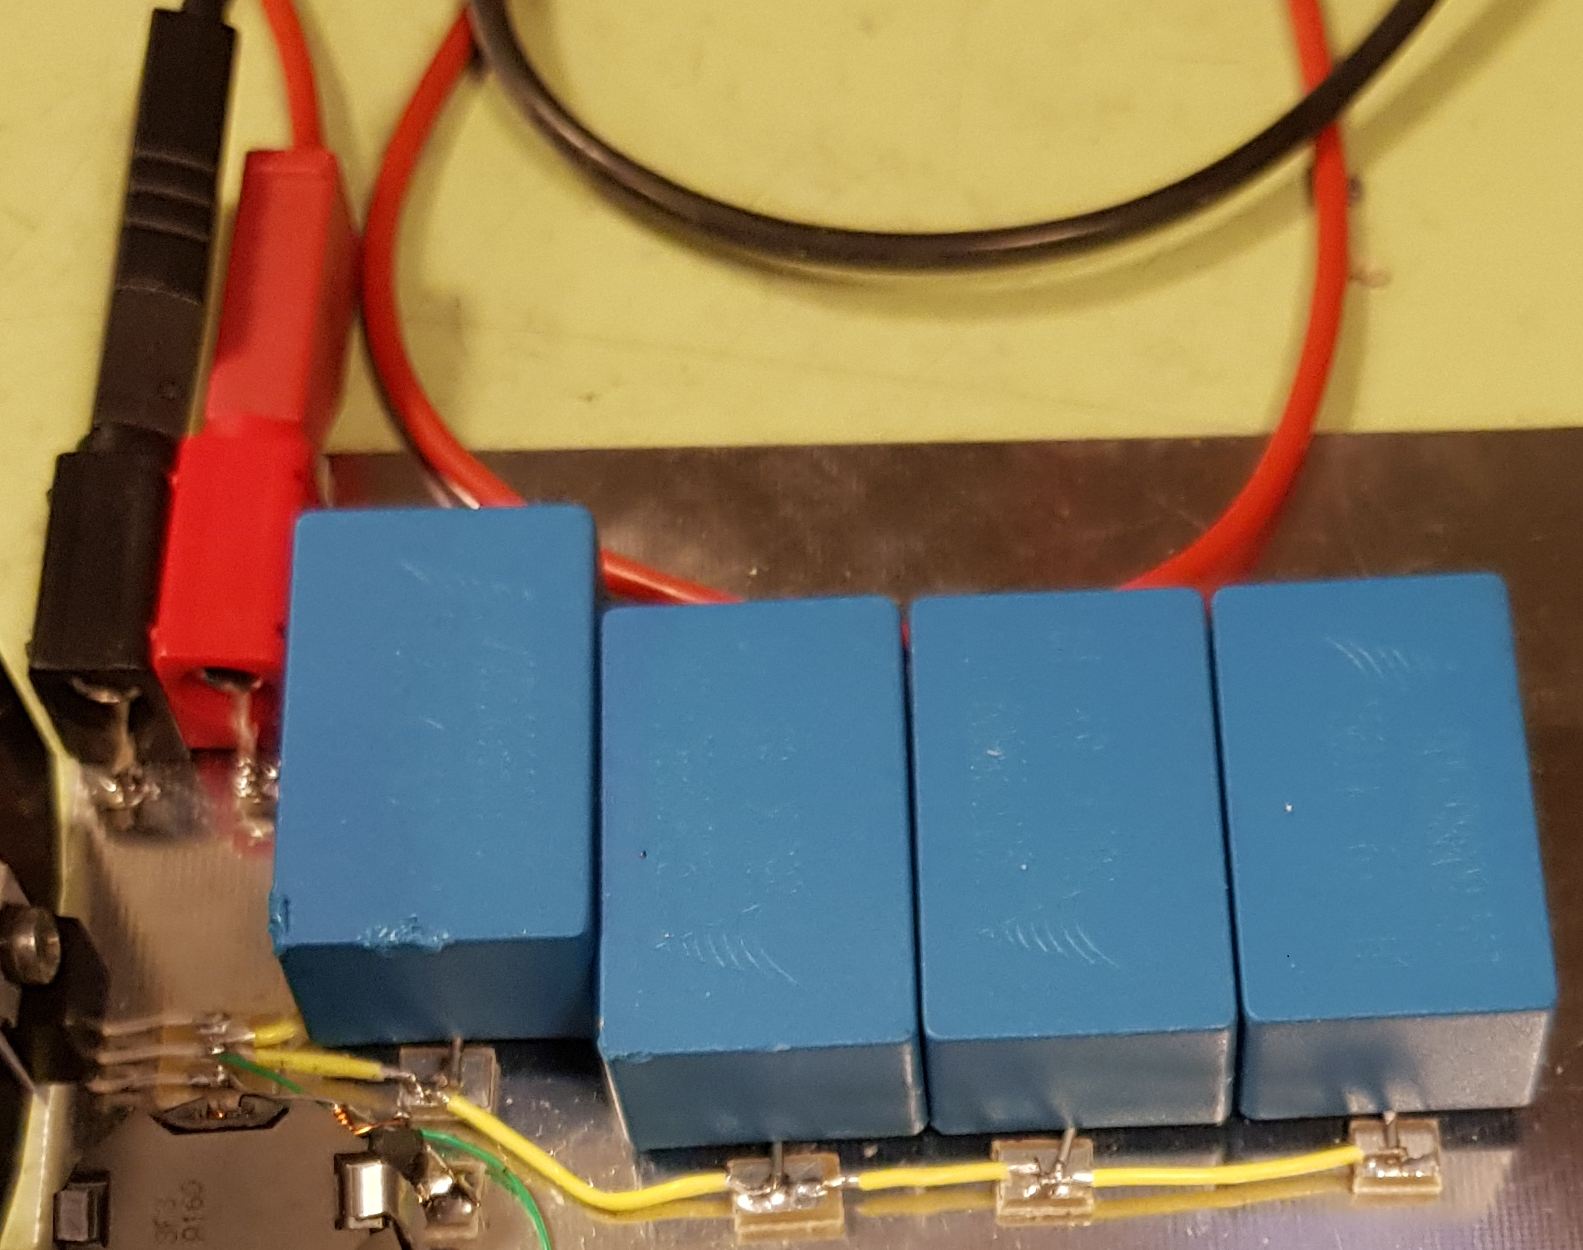
\includegraphics[width=0.5\linewidth]{../Dokumentation/tex/3iteration/Billeder/Analyse/Udgangsfilter_2iteration.png}
	\caption{Realisering af udgangsfilter efter 2. iteration}
	\label{fig:udgangsfilter}
\end{figure}

\noindent En nærmere analyse af udgangsfilteret er beskrevet i dokumentationens afsnit 6.4.


\subsection{Regulering}
Efter 2. iteration blev besluttet at optimere converterens båndbredde, da der var en stor margin til kravene for både gain- og fasemargin. Med en større båndbredde, ville der samtidig opnås en hurtigere responstid i systemet. 

For design af det nye kompensationsnetværk, blev der taget udgangspunkt i bode plottet for power-modulet. Ud fra kravene for converterens stabilitet, kunne det ses, at der kunne tilføres en forstærkning på $8.6\decibel$, og stadig overholde kravene for gain- og fasemargin. Samtidig blev knækfrekvensen for fejlforstærkeren flyttet til $132.8\hertz$, da den dominerende pol for converteren lå her. 

For at opnå den ønskede forstærkning på $8.6\decibel$, eller $2.66gg$, regnes modstanden i kompensationsnetværket til $R_{comp} = 49.8k\ohm$. For at opnå den valgte knækfrekvens regnes kondensatoren til $24.2nF$. 

For en mere detaljeret gennemgang af overføringsfunktionernes indhold, og deres bode plots, henvises til dokumentationens afsnit 6.5 og 6.8.5.


\section{Tab}
Dette afsnit omhandler de overvejelser, der er gjort omkring tab i 2. iteration. Her omtales hvilke bidrag, der er taget højde for, til udberegninger af tab for de enkelte komponenter. Udregningerne og yderligere forklaring af disse, kan findes dokumentationen afsnit 5.7.

\subsubsection{Transformator}
Tabet i transformatoren er set som to dele. Et kernetab og et kobbertab. Kernetabet afhænger af  kernematerialet, selvinduktionen og strømmen i viklingerne. Disse bruges til at udregne fluxen i kernen. Med denne værdi og databladskurven for det specifikke tab som funktion af maks flux massefylden, er kernetabet blevet estimeret. 

Kobbertabet kommer af modstanden, der er i kobbertrådene, som er viklet om kernen. Dette indebærer både bidrag fra en DC modstand og en AC modstand. DC modstanden er udregnet ud fra længden og tykkelsen af kobbertrådene. AC modstanden opstår på grund af magnetfeltet kobbertrådene ligger i. AC modstandens del af kobbertabet er der i dette projket ikke valgt at tage højde for.

Det samlede tab for transformatoren er testet, ved at måle temperaturen på kernen efter converteren har været i gang over længere tid. Med en datablads værdi af den termiske modstand for en RM8 kerne er tabet herefter udregnet.   

\subsubsection{MOSFET}
MOSFET'ens tab kan ligeledes deles op i to centrale bidrag; 

conduction tab og switchtab. Conduction tabet kommer af RMS strømmen der løber i MOSFET'ens ON modstand. 

Switchtabet kommer som konsekvens af effekttrekanterne, der opstår, imellem MOSFET'ens ON og OFF perioder. Effekttrekanterne er i dette projekt estimeret ved at udregne dem som arealet af to lige store trekanter. Højden på trekanten er peakaverage strømmen ganget med den maksimale spænding der vil ligge over MOSFET'en. Længden af trekanten fås af den samlede switch-tid i forhold til den samlede switch periode. 

Det samlede tab i MOSFET'en er testet ved at måle temperaturen på kølepladen efter converteren har været i gang over længere tid. Denne temperaturstigning ganget med køle-koefficienten for kølepladen giver tabet. 

\subsubsection{Diode}
Tabet i dioden er udregnet ved, at kigge på spændingsfaldet over dioden ganget udgangsstrømmen. Som nævnt benyttes en schottky diode, og der har derfor ikke været behov for betragtninger af switch-tabet i dioden. 

Tabet for dioden er fundet ved at måle temperaturen af kølepladen ligesom ved MOSFET'en ovenfor.   

\subsubsection{Kondensator}
Med en kendt ESR modstand for kondensatoren, har det været muligt at beregne tabet i denne. Da modstanden er så lille, er tabet dog uden betydning for det samlede tab.

\subsubsection{Current-sence tab}
Tabet i current-sence modstanden er udregnet ved modstandsværdien ganget med RMS strømmen i anden. Strømmen i igennem modstanden er den samme som løber i den primære vikling. 

\subsubsection{Samlet tab}
De ovenstående tab er alle analyseret og simuleret. Derudover er der lavet test af de tab, hvor det var muligt. Resultatet af dette ses i resultatafsnittet \fxnote{indsæt resultatafsnit for tab}.
Det samlede tab for converteren i 2. iteration er i analyse og simulering fundet ved at lægge de fundne tab sammen. I testen er der set på den effekt der sendes ind i converteren og trukket udgangseffekten fra denne.



\section{Integrationstest} \label{Integrationstest}
Der er lavet tre forskellige test af det samlede system, til at teste de essentielle funktioner af converteren. Det drejer sig om constant-load, gain-fase måling og load-step. For nærmere beskrivelse af hver enkelt test, henvises til dokumentationen afsnit 5.9.

På figur~\ref{fig:sche2iteration} ses et schematic for det samlede implementerede kredsløb for 2. iteration.
\begin{figure}[H]
	\center
	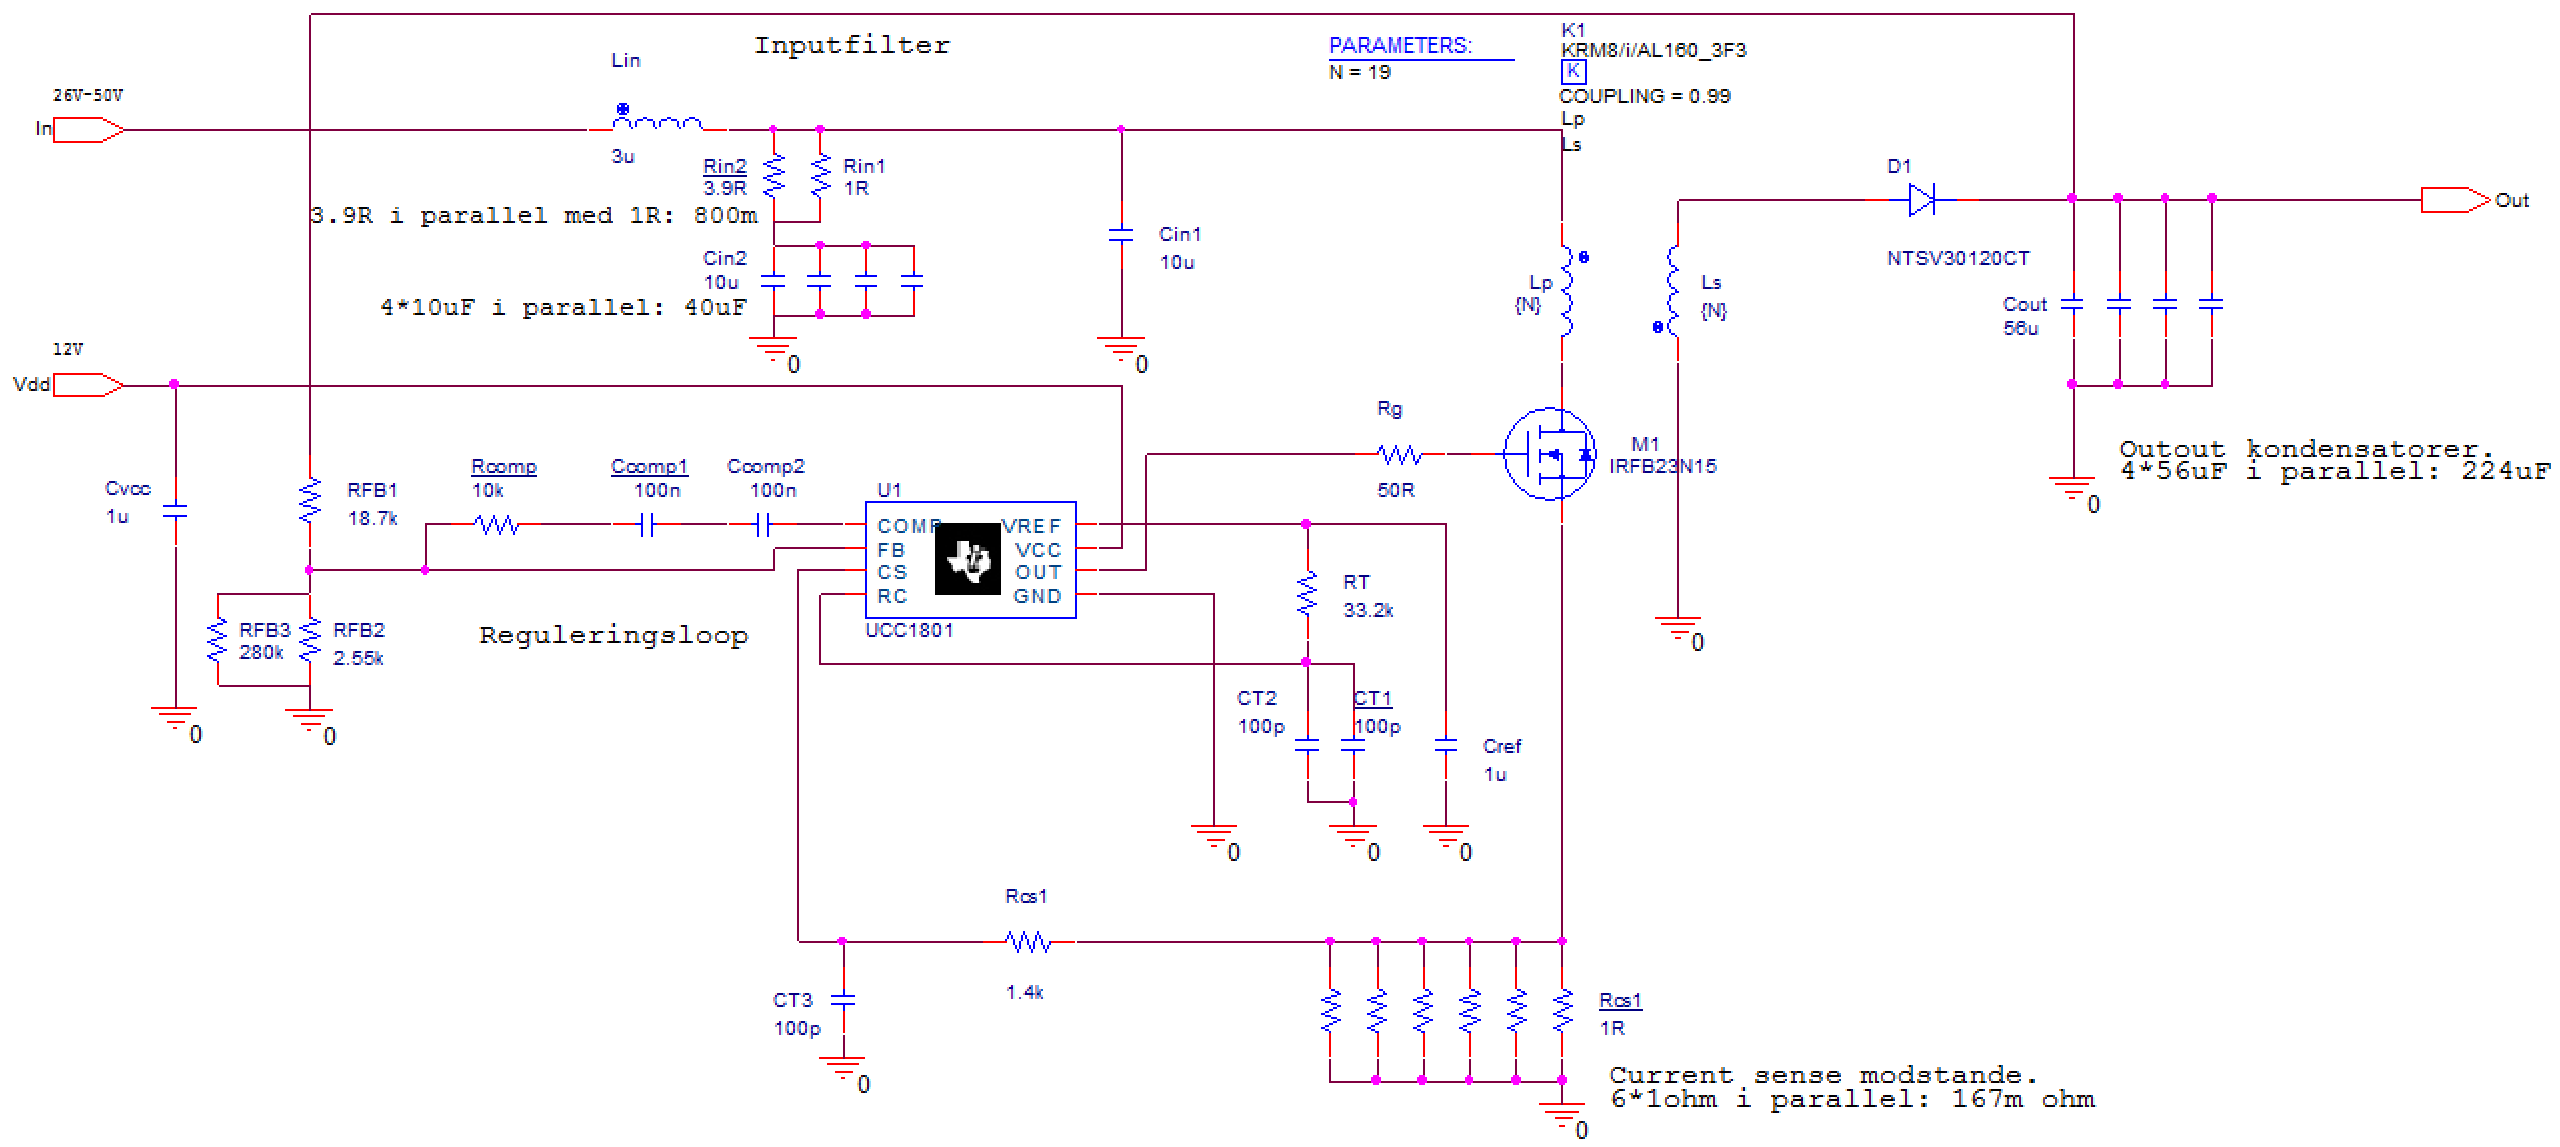
\includegraphics[max width=1.1\linewidth]{../dokumentation/tex/2iteration/billeder/Schemaricoverview_2iteration.PNG}
	\caption{Schematic overblik for 2. iteration}
	\label{fig:sche2iteration}
\end{figure}

\subsection{Constant-load}
Ved testen constant-load måles interessante steder i systemet, hvor en konstant belastning bruges. Her er en belastning på $8.4\ohm$ benyttet, med en indgangsspænding på 26V, med mindre andet er opgivet.

Ved testen er spændingen over outputtet, MOSFET'en og dioden målt. Desuden er der lavet målinger på de centrale dele af PWM-controlleren. Det indebærer målinger af switch-frekvensen, switch-tiden og stigetiden på filtret til current-sense signalet.  
Ved testen er converterens tab samtidig fundet. Tabet for transformator, MOSFET og diode er fået ved at måle temperaturen af den enkelte komponent, efter converteren har været kørende i længere tid. Temperaturstigningen er sammen med kølepladernes kølekoefficienter, og transformatorens termiske modstand, brugt til beregning af tab. Det samlede tab for converteren i 2. iteration, er i analyse og simulering fundet ved, at lægge de fundne tab sammen. I testen er der set på den effekt, der sendes ind i converteren og trukket udgangseffekten fra denne.

\subsection{Gain-fase måling}
Til gain-fase måling af converteren er Network Analyzeren HP4194A\cite{hp4194} benyttet. Her laves en måling af overføringsfunktionen for power-modul, fejlforstærker og for det samlede system. Det er gjort, ved at indføre et fejlsignal i tilbagekoblingen, og måle hvordan udgangen ændrer sig. Fejlsignalet blev indført med en amplitude på $30mV$. Dette er der lavet et frekvens-sweep på fra, $10\Hz$ til $100kHz$. Målingerne fra Network Analyzeren overføres til et Excel ark, hvor et bode plot er udarbejdet ud fra testmålingerne. 

\subsection{Load-step}
For at lave load-step testen, er der som udgangsbelastning brugt to $20\ohm$ modstande i parallel. Den ene koblet til en switch, så den kan kobles til eller fra. Det gør, at når switchen er OFF, består belastningen af en $20\ohm$ modstand. Når switchen er ON, består den i stedet af en $10\ohm$ modstand. Switchen var indstillet til at sende en puls på 10ms.

\noindent Ved denne test er det spændingsændringen på outputtet der er målt.


%%% Første iteration
	% Converter
	
%%% Anden iteration
	% Transformator
	% PWM controller
	% MOSFET, diode og udgangsfilter
	% Regulering
	% Tab
	
%%% Tredje iteration
	% Snubber
	% Switch-tid
	% Udgangsfilter
	% Regulering
	% Tab

	
	
	
	\printbibliography[title={Litteraturliste}]

\end{document}